% Options for packages loaded elsewhere
\PassOptionsToPackage{unicode}{hyperref}
\PassOptionsToPackage{hyphens}{url}
%
\documentclass[
]{article}
\usepackage{amsmath,amssymb}
\usepackage{lmodern}
\usepackage{iftex}
\ifPDFTeX
  \usepackage[T1]{fontenc}
  \usepackage[utf8]{inputenc}
  \usepackage{textcomp} % provide euro and other symbols
\else % if luatex or xetex
  \usepackage{unicode-math}
  \defaultfontfeatures{Scale=MatchLowercase}
  \defaultfontfeatures[\rmfamily]{Ligatures=TeX,Scale=1}
\fi
% Use upquote if available, for straight quotes in verbatim environments
\IfFileExists{upquote.sty}{\usepackage{upquote}}{}
\IfFileExists{microtype.sty}{% use microtype if available
  \usepackage[]{microtype}
  \UseMicrotypeSet[protrusion]{basicmath} % disable protrusion for tt fonts
}{}
\makeatletter
\@ifundefined{KOMAClassName}{% if non-KOMA class
  \IfFileExists{parskip.sty}{%
    \usepackage{parskip}
  }{% else
    \setlength{\parindent}{0pt}
    \setlength{\parskip}{6pt plus 2pt minus 1pt}}
}{% if KOMA class
  \KOMAoptions{parskip=half}}
\makeatother
\usepackage{xcolor}
\usepackage[margin=1in]{geometry}
\usepackage{longtable,booktabs,array}
\usepackage{calc} % for calculating minipage widths
% Correct order of tables after \paragraph or \subparagraph
\usepackage{etoolbox}
\makeatletter
\patchcmd\longtable{\par}{\if@noskipsec\mbox{}\fi\par}{}{}
\makeatother
% Allow footnotes in longtable head/foot
\IfFileExists{footnotehyper.sty}{\usepackage{footnotehyper}}{\usepackage{footnote}}
\makesavenoteenv{longtable}
\usepackage{graphicx}
\makeatletter
\def\maxwidth{\ifdim\Gin@nat@width>\linewidth\linewidth\else\Gin@nat@width\fi}
\def\maxheight{\ifdim\Gin@nat@height>\textheight\textheight\else\Gin@nat@height\fi}
\makeatother
% Scale images if necessary, so that they will not overflow the page
% margins by default, and it is still possible to overwrite the defaults
% using explicit options in \includegraphics[width, height, ...]{}
\setkeys{Gin}{width=\maxwidth,height=\maxheight,keepaspectratio}
% Set default figure placement to htbp
\makeatletter
\def\fps@figure{htbp}
\makeatother
\setlength{\emergencystretch}{3em} % prevent overfull lines
\providecommand{\tightlist}{%
  \setlength{\itemsep}{0pt}\setlength{\parskip}{0pt}}
\setcounter{secnumdepth}{5}
\usepackage{booktabs}
\ifLuaTeX
  \usepackage{selnolig}  % disable illegal ligatures
\fi
\usepackage[]{natbib}
\bibliographystyle{plainnat}
\IfFileExists{bookmark.sty}{\usepackage{bookmark}}{\usepackage{hyperref}}
\IfFileExists{xurl.sty}{\usepackage{xurl}}{} % add URL line breaks if available
\urlstyle{same} % disable monospaced font for URLs
\hypersetup{
  hidelinks,
  pdfcreator={LaTeX via pandoc}}

\author{}
\date{\vspace{-2.5em}2024-05-31}

\begin{document}

{
\setcounter{tocdepth}{2}
\tableofcontents
}
\hypertarget{project-management-handbook}{%
\section{\texorpdfstring{\textbf{Project Management Handbook}}{Project Management Handbook}}\label{project-management-handbook}}

\hypertarget{history-of-changes}{%
\subsection{History of Changes}\label{history-of-changes}}

\begin{itemize}
\tightlist
\item
  Change of PM\\
\item
  Deliverable review timeline
\end{itemize}

\begin{longtable}[]{@{}
  >{\raggedright\arraybackslash}p{(\columnwidth - 6\tabcolsep) * \real{0.2055}}
  >{\raggedright\arraybackslash}p{(\columnwidth - 6\tabcolsep) * \real{0.2055}}
  >{\raggedright\arraybackslash}p{(\columnwidth - 6\tabcolsep) * \real{0.2055}}
  >{\raggedright\arraybackslash}p{(\columnwidth - 6\tabcolsep) * \real{0.3836}}@{}}
\toprule()
\endhead
\textbf{Date} & & \textbf{Page/section} & \textbf{Nature of change and reason / justification of change proposed} \\
\textbf{Change of project manager} & 07 May 2024 & Throughout & Our named project manager changed from Marina Mattera to Rebecca Fischer -- this is has been reflected throughout the document \\
\textbf{Change in Steering Committee} & 07 May 2024 & & \\
\bottomrule()
\end{longtable}

\hypertarget{list-of-abbreviations}{%
\subsection{List of Abbreviations}\label{list-of-abbreviations}}

\begin{longtable}[]{@{}
  >{\raggedright\arraybackslash}p{(\columnwidth - 2\tabcolsep) * \real{0.2639}}
  >{\raggedright\arraybackslash}p{(\columnwidth - 2\tabcolsep) * \real{0.7361}}@{}}
\toprule()
\endhead
D & Deliverable \\
DMP & Data Management Plan \\
DoA & Description of the Action \\
DoW & Description of Work \\
EC & European Commission \\
EU & European Union \\
GA & Grant Agreement \\
M & Month \\
MS & Milestone \\
OSIRIS & Open Science to Increase Reproducibility in Science \\
PC & Project Coordinator \\
PM & Project Manager \\
PMO & Project Management Office \\
PU & Public \\
R & Report \\
SEAB & Scientific and Ethical Advisory Board \\
SERI & Swiss State Secretariat for Education \\
SC & Steering Committee \\
SMART & Specific, Measurable, Achievable, Relevant, and Time-bound \\
UKRI & United Kingdom Research and Innovation \\
TIER2 & Enhancing Trust, Integrity and Efficiency in Research through next-level Reproducibility \\
WP & Work Package \\
\bottomrule()
\end{longtable}

\hypertarget{list-of-linked-irise-resources}{%
\subsection{List of linked iRISE resources}\label{list-of-linked-irise-resources}}

\begin{itemize}
\item
  \href{https://charitede.sharepoint.com/sites/iRISE/Shared\%20Documents/Forms/AllItems.aspx}{iRISE SharePoint}
\item
  \href{https://teams.microsoft.com/l/team/19\%3aBeyH-eKopgikP84hU4FuJggrTXugFiipnYUq8krUnAE1\%40thread.tacv2/conversations?groupId=63cd0d10-aa1b-4db9-9bb0-ed23b58ec69b\&tenantId=afe91939-923e-432c-bc66-cbc3ec18d02c}{iRISE Microsoft Teams}
\item
  \href{https://charitede.sharepoint.com/:f:/r/sites/iRISE/Shared\%20Documents/General/Grant\%20Agreement/AMD-101094853-4_Nov2023?csf=1\&web=1\&e=cuFpdE}{iRISE Grant Agreement}
\item
  \href{https://charitede.sharepoint.com/:b:/r/sites/iRISE/Shared\%20Documents/General/Grant\%20Agreement/GA\%20amendment\%20Sept.\%202023/iRISE_Annex1B_DoA_2023-09-25_v4_clean.pdf?csf=1\&web=1\&e=CGlIBC}{Description of Action}
\item
  \href{https://charitede.sharepoint.com/:w:/r/sites/iRISE/Shared\%20Documents/General/iRISE\%20Mailing\%20List\%20Full.docx?d=w78aadfc66f9b4bdc878dd41138496398\&csf=1\&web=1\&e=xnGHy4}{Mailing List}
\item
  \href{https://www.zotero.org/groups/5148075/irise_library}{iRISE Zotero Library}
\item
  \href{https://charitede.sharepoint.com/:x:/r/sites/iRISE/Shared\%20Documents/WP6/iRISE\%20Dissemination\%20Activity\%20Record.xlsx?d=w47a1cbfaa6c34ab5aee84a6dba643912\&csf=1\&web=1\&e=9cfBaW}{Dissemination Activity Record}
\item
  \href{https://charitede.sharepoint.com/:w:/r/sites/iRISE/Shared\%20Documents/WP6/iRISE\%20Dissemination\%20Plan_Draft\%201.2.docx?d=w7a63d0ea4a374c1bbe3b7fd98d0c7d2f\&csf=1\&web=1\&e=jY54DT}{Dissemination, Exploitation, and Communication Plan}
\item
  \href{https://charitede.sharepoint.com/:f:/r/sites/iRISE/Shared\%20Documents/Branding\%20and\%20Website/iRISE\%20Logos/Logos?csf=1\&web=1\&e=mh7pQM}{iRISE Logos}
\item
  \href{https://charitede.sharepoint.com/:f:/r/sites/iRISE/Shared\%20Documents/General/iRISE\%20Dissemination_Communication_Templates/Templates?csf=1\&web=1\&e=P8QVBa}{Templates Folder}

  \begin{itemize}
  \item
    \href{https://charitede.sharepoint.com/:p:/r/sites/iRISE/Shared\%20Documents/General/iRISE\%20Dissemination_Communication_Templates/Templates/PPT\%20Template.pptx?d=w197f096e83fa4576a6f82bdcd51489b2\&csf=1\&web=1\&e=MREwQ4}{PowerPoint}
  \item
    \href{https://charitede.sharepoint.com/:w:/r/sites/iRISE/Shared\%20Documents/General/iRISE\%20Dissemination_Communication_Templates/Templates/DocTemplate.docx?d=wcb083ece13604791b342b0bb693fe067\&csf=1\&web=1\&e=f61QPR}{Word Docs}
  \item
    \href{https://charitede.sharepoint.com/:u:/r/sites/iRISE/Shared\%20Documents/Branding\%20and\%20Website/iRISE.thmx?csf=1\&web=1\&e=fyKrZL}{PowerPoint Theme}
  \item
    \href{https://charitede.sharepoint.com/:w:/r/sites/iRISE/Shared\%20Documents/General/iRISE\%20Dissemination_Communication_Templates/Templates/DeliverableTemplate.docx?d=w4ec2474158ab425f86655df0f923297d\&csf=1\&web=1\&e=drgFm9}{Deliverable Template}
  \end{itemize}
\item
  \href{https://charitede.sharepoint.com/:f:/r/sites/iRISE/Shared\%20Documents/General/Project\%20Outputs\%20(Deliverables,\%20Milestones,\%20Papers)/Deliverables\%20submitted?csf=1\&web=1\&e=L4NinF}{Deliverables Submitted Folder}
\item
  \href{https://tasks.office.com/charitede.onmicrosoft.com/en-US/Home/Planner/\#/plantaskboard?groupId=63cd0d10-aa1b-4db9-9bb0-ed23b58ec69b\&planId=P4fliqzuUEeyiZo6z3Z3L5YAAegq}{iRISE Project Management Planner}
\item
  \href{https://charitede.sharepoint.com/:f:/r/sites/iRISE/Shared\%20Documents/WP7/Project\%20Management/Risk\%20Assessments?csf=1\&web=1\&e=v2Nm3v}{Risk Assessment folder}
\end{itemize}

\hypertarget{introduction}{%
\section{\texorpdfstring{\textbf{Introduction}}{Introduction}}\label{introduction}}

Our vision, in iRISE, is to deepen understanding of reproducibility drivers, evaluate their effectiveness and provide concrete solutions to enhance scientific evidence. We will foster a research culture of openness, integrity, and trustworthiness to advance reproducibility and knowledge.

\hypertarget{background}{%
\subsection{Background}\label{background}}

Reproducibility is a complex and multifaceted phenomenon that encompasses a continuum of practices related to the reproduction and replication of scientific results. iRISE takes an integrated approach to understanding, investigating and guiding strategies to address irreproducibility.

\hypertarget{objectives}{%
\subsection{Objectives}\label{objectives}}

Our objectives are to:

\begin{enumerate}
\def\labelenumi{\arabic{enumi}.}
\tightlist
\item
  develop working definitions and a general framework for diagnosing and addressing reproducibility problems, define costs, benefits and opportunities, and assess the utility of theoretical evidence in forecasting the success of interventions (WP1),\\
\item
  perform scoping and systematic reviews to identify and evaluate existing interventions to improve reproducibility (WP2),\\
\item
  explore the interface between reproducibility and research culture, and in particular considerations and mainstreaming of equity, diversity, and inclusion (EDI) (WP3),\\
\item
  consult and engage key stakeholder groups in prioritising practices and practical tool development for adoption to increase reproducibility (WP4),\\
\item
  test efficacy and feasibility of specific interventions to increase reproducibility (WP5),\\
\item
  curate and integrate these different types of evidence to increase reproducibility for dissemination and implementation (WP6) and\\
\item
  effectively project manage iRISE to achieve our objectives in a timely manner within budget (WP7).
\end{enumerate}

\hypertarget{importance-of-effective-project-management}{%
\subsection{Importance of effective project management}\label{importance-of-effective-project-management}}

iRISE involves multiple partners, disciplines and objectives. We need to coordinate and manage our interactions to ensure:

\begin{enumerate}
\def\labelenumi{\arabic{enumi}.}
\tightlist
\item
  We progress in a timely manner, meeting milestones and deliverables\\
\item
  We facilitate effective communication and engagement within and outside the consortium\\
\item
  Our work is rigorous, maintaining high-quality outputs and conduct\\
\item
  We foster collaboration to enable us to work together smoothly despite geographical and disciplinary differences\\
\item
  We promote accountability by clearly defining roles, responsibilities and tasks. This will include thorough documentation which is essential for reporting and future reference
\end{enumerate}

Project management is the backbone that will hold us together. It ensures that the diverse elements of the project work harmoniously toward achieving our objectives, maximising impact, and delivering outcomes on time and within budget.

\hypertarget{purpose-and-structure-of-this-handbook}{%
\subsection{Purpose and structure of this handbook}\label{purpose-and-structure-of-this-handbook}}

This handbook provides practical insights and step-by-step guidance for the Project Management Office (PMO) and consortium members to ensure the successful execution of iRISE. All partners of the consortium should refer to this handbook throughout the duration of the project.\\
The handbook is designed to align with EU regulations, guidelines, and best practices relevant to project management and is structured as follows:

\begin{itemize}
\tightlist
\item
  \protect\hyperlink{project-overview}{Project Overview}\\
\item
  \protect\hyperlink{consortium-structure}{Consortium Structure}\\
\item
  \protect\hyperlink{communication-and-reporting}{Communication and Reporting}\\
\item
  \protect\hyperlink{data-and-file-management}{Data and File Management}\\
\item
  \protect\hyperlink{reporting-to-the-european-commission}{Reporting to the European Commission}\\
\item
  \protect\hyperlink{deliverable-management-and-quality-assurance}{Deliverable Management and Quality Assurance}\\
\item
  \protect\hyperlink{overview-of-key-dates}{Overview of Key Dates}\\
\item
  \protect\hyperlink{intellectual-property-and-dissemination}{Intellectual Property and Dissemination}\\
\item
  \protect\hyperlink{ethics-and-compliance}{Ethics and Compliance}\\
\item
  \protect\hyperlink{appendix-1-ethical-self-assessment-and-ethical-risks-identification}{Appendices}
\end{itemize}

The content is intended to help members and the project adhere to EU requirements and maximise our chances of executing a successful project.\\
The handbook will be stored on the \href{https://charitede.sharepoint.com/sites/iRISE/Shared\%20Documents/Forms/AllItems.aspx}{iRISE SharePoint} and will act as a living document, updated periodically to reflect any required changes. References to other documents are via file links to the iRISE SharePoint to ensure that information is up-to-date and a list of the documents linked is provided at the end of the book.\\
Please contact Sarah McCann (\href{mailto:sarah.mccann@bih-charite.de}{\nolinkurl{sarah.mccann@bih-charite.de}}), Emily Sena (\href{mailto:emily.sena@ed.ac.uk}{\nolinkurl{emily.sena@ed.ac.uk}}) or Rebecca Fischer (\href{mailto:rebecca.fischer@uni-jena.de}{\nolinkurl{rebecca.fischer@uni-jena.de}}) if you have any enquires or need support related to the handbook.

\hypertarget{project-overview}{%
\section{\texorpdfstring{\textbf{Project Overview}}{Project Overview}}\label{project-overview}}

iRISE consists of 15 partners, from nine countries and includes 37 members. The iRISE partners are Universitaetsmedizin Berlin (CHARITE), Sveuciliste U Splitu Medicinski Fakultet (MEFST), Karolinska Institutet (KI), Stichting Radboud Universitair Medisch Centrum (RUMC), Eatris Eric (EATRIS), Helsingin Yliopisto (UH), Miller International Knowledge Sl (MIK), University Of Cyprus (UCY), Guarantors Of Eqipd E.V. (GOEQIPD), Tilburg University (TiU), Universiteit Maastricht (UMAAS), Universitaet Zurich (UZH), Universitaet Bern (UBERN), Heriot Watt University (HW), The University Of Edinburgh (UEDIN).\\
iRISE receives funding from the European Union's Horizon Europe research and innovation programme under grant agreement No 101094853. The project also receives funding from UK Research and Innovation (UKRI) and the Swiss State Secretariat for Education, Research and Innovation (SERI): Direct Funding for Collaborative Projects as part of the transitional measures.

\hypertarget{horizon-europe-framework}{%
\subsection{Horizon Europe Framework}\label{horizon-europe-framework}}

Horizon Europe is the European Union's framework program for research and innovation. It aims to address societal challenges, promote scientific excellence, and drive economic growth and competitiveness in Europe. The program supports research and innovation activities across various fields, including but not limited to health, environment, digital technologies, and social sciences. Horizon Europe's objectives include:

\begin{itemize}
\tightlist
\item
  \textbf{Excellence in Research}: Enhancing Europe's research and innovation capacities by fostering scientific excellence and breakthrough discoveries.
\item
  \textbf{Global Challenges and Industrial Competitiveness}: Addressing pressing global challenges, such as climate change, health, and digitalization, while boosting the competitiveness of European industries.
\item
  \textbf{Open Science and Open Innovation}: Promoting open access to research results, data, and publications to accelerate knowledge sharing and collaboration.
\item
  \textbf{Innovative Partnerships}: Establishing partnerships between academia, industry, and other stakeholders to drive innovation and address real-world challenges.
\end{itemize}

\hypertarget{grant-agreement}{%
\subsection{Grant Agreement}\label{grant-agreement}}

Projects funded under Horizon Europe are governed by grant agreements between the European Commission and the project consortium. These agreements outline the terms and conditions of the funding and the responsibilities of all parties involved. A copy of the \href{https://charitede.sharepoint.com/:f:/r/sites/iRISE/Shared\%20Documents/General/Grant\%20Agreement/AMD-101094853-4_Nov2023?csf=1\&web=1\&e=cuFpdE}{iRISE Grant Agreement} can be found in the iRISE SharePoint.

\hypertarget{horizon-europe-call}{%
\subsection{Horizon Europe Call}\label{horizon-europe-call}}

iRISE is funded under Horizon Europe Framework Programme (HORIZON):
Call: European Research Area HORIZON-WIDER A-2022-ERA-01)
TOPIC ID: HORIZON-WIDERA-2022-ERA-01-41; \href{https://ec.europa.eu/info/funding-tenders/opportunities/portal/screen/opportunities/topic-details/horizon-widera-2022-era-01-41}{Increasing the reproducibility of scientific results}

\hypertarget{consortium-structure}{%
\section{\texorpdfstring{\textbf{Consortium Structure}}{Consortium Structure}}\label{consortium-structure}}

iRISE has established a well-defined project management and governance
structure to ensure the efficient organization of the project,
facilitate decision-making processes, and foster collaboration in line
with the project's description of action. Our consortium management
structure consists of the following key roles:\\

\textbf{Project Coordinators}: iRISE is co-coordinated by \textbf{Dr Sarah McCann
(Charité)} and \textbf{Professor Emily Sena (UEDIN)}. McCann and Sena are
responsible for overseeing the project as a whole, ensuring alignment
with its objectives, maintaining quality, adhering to the project
schedule, and managing the budget. Additionally, McCann, as the
designated coordinator in the Grant Agreement, serves as the primary
contact point for the European Commission.\\
Supported by the Project Management Office (PMO), the BIH QUEST Center
Office Administration Team, and the Research Grants Office at Charité,
the co-coordinator's main responsibilities are to: (1) ensure efficient
project management; (2) guide the project's decision-making process; (3)
alternate chairing of the Steering Committee and lead the set of
activities to be carried out by this committee; (4) coordinate
technical/support activities across work-packages; (5) maintain and
regularly update the contents of this project management handbook to
support quality and timely delivery of iRISE deliverables; and (6) act
as the Financial Officer within the Consortium, including managing the
preparation of financial statements for the Commission.\\

\textbf{Project Manager (Rebecca Fischer, MIK)}: The Project Manager is
responsible for the day-to-day coordination and administration of the
project. She will ensure that the management procedures as defined below
are carried out throughout the project's lifetime and that supporting
tools and templates will be made available. Management tasks include
consolidation of the project planning, progress reports, milestone
monitoring, financial management, etc. by gathering and aggregating
inputs from the project partners. The project manager should be the
first point of contact for project iRISE enquiries and will direct
enquiries to the relevant persons or information sources.\\

\textbf{Project Management Office (PMO)}: The PMO, consists of the
Co-coordinators (McCann and Sena) and the Project Manager (Fischer). The
PMO will work collectively to successfully manage the project to meet
our objectives, milestones and deliverables. They are responsible for
financial management, modifications to the grant or consortium
agreements and collecting information for the purposes of reporting to
the European Commission. The PMO is also responsible for the
organisation of project meetings, including ensuring work package and
steering committee meetings are held, and the planning and chairing of
the annual iRISE General Assembly. The PMO will meet at least monthly to
ensure its effective performance.\\

\textbf{Steering Committee (SC)}: Comprising eight members, the iRISE SC
includes each of the work package leads: \textbf{McCann} (Charité), \textbf{Sena}
(UEDIN), \textbf{Heyard} (UZH), \textbf{Fanelli} (HW), \textbf{Wever} (RUMC),
\textbf{Marušić} (MFEST), \textbf{Miller} (MIK) and \textbf{Currie} (UEDIN). The SC is
responsible for the implementation of the project, quality management
and is the highest decision-making body of the consortium. The main
responsibilities of the SC include: (1) the definition of the overall
project strategy; (2) fulfilling the Commission requirements pertaining
to preparation of progress and financial reports; (3) deciding on
long-term exploitation plans; (4) conflict resolution within the
Consortium, in line with the details described in the iRISE Conflict
Resolution Policy; (5) technical coordination and decision-making
(assessment of the technical work, interchange of technical information
amongst partners, submission of deliverables, etc.); and (6) risk
management. The SC will meet quarterly, requires 2/3 majority for
quorum, with decisions reached through a simple majority process.\\

\textbf{Work Package (WP) Leads}: iRISE comprises seven WPs, each led by 1-2
individuals. The leads are:\\

\begin{itemize}
\tightlist
\item
  WP1 - \textbf{Heyard} (UZH), \textbf{Fanelli} (HW),
\item
  WP2 and WP7 - \textbf{McCann} (Charité), \textbf{Sena} (UEDIN),
\item
  WP3 - \textbf{Miller} (MIK),
\item
  WP4 - \textbf{Marušić} (MFEST),
\item
  WP5 - \textbf{Wever} (RUMC), and
\item
  WP6 - \textbf{Currie} (UEDIN).
\end{itemize}

WP leads are responsible for ensuring the delivery of their WP
objectives. They are responsible for implementing and managing tasks and
providing guidance and support to task leads as appropriate. They are
responsible for ensuring regular, timely and effective communication
between all members of the WP, including the organisation and chairing
of WP meetings. They oversee the risk management for all tasks within
the work package and are responsible for all technical aspects of their
WP (meeting of milestones, timely submission of deliverables and
reports, and the quality assurance of all WP outputs). WP leads also
provide reports back to steering committee.\\

\textbf{Task Leaders}: Work within WPs is divided into tasks with designated
task leaders. Task leaders are responsible for the technical management
of specific activities, including planning, monitoring and reporting to
the WP leader. Each individual partner holds ultimate responsibility for
the technical and administrative outputs assigned to them.\\

\begin{longtable}[]{@{}
  >{\raggedright\arraybackslash}p{(\columnwidth - 4\tabcolsep) * \real{0.1972}}
  >{\raggedright\arraybackslash}p{(\columnwidth - 4\tabcolsep) * \real{0.6056}}
  >{\raggedright\arraybackslash}p{(\columnwidth - 4\tabcolsep) * \real{0.1972}}@{}}
\toprule()
\begin{minipage}[b]{\linewidth}\raggedright
WP
\end{minipage} & \begin{minipage}[b]{\linewidth}\raggedright
\textbf{Task}
\end{minipage} & \begin{minipage}[b]{\linewidth}\raggedright
\textbf{Lead}
\end{minipage} \\
\midrule()
\endhead
\textbf{1} & 1.1 Background scoping and framing & Bernhard Voelkl \\
& 1.2 Modelling irreproducibility causes and remedies & Daniele Fanelli \\
& 1.3 Validating statistical methods to assess and improve reproducibility & Rachel Heyard \\
& 1.4 Empirical meta-meta-studies & Rachel Heyard \\
& 1.5 Testing meta-scientific predictions & Daniele Fanelli \\
\textbf{2} & 2.1 Create a Systematic Online Living Evidence Summary (SOLES) of candidate interventions & Kaitlyn Hair \\
& 2.2 Perform systematic reviews of interventions that have been evaluated for effectiveness & Sarah McCann \\
& 2.3 Develop a framework to evaluate candidate reproducibility interventions & Carlijn Hooijmans \\
\textbf{3} & 3.1 To provide a cross-cutting ``support service'' that lends a research culture and EDI lens to other WPs & Stephanie Zellers \\
& 3.2 Identifying areas of underrepresentation in research practitioners and participants & Katharina Miller \\
& 3.3 Defining the characteristics of those currently engaged in reproducible research & Maia Salholz-Hillel \\
& 3.4 Develop a framework to determine the EDI impacts of interventions & Maia Salholz-Hillel \\
& 3.5 Explore how EDI considerations intersect with diversity of research culture & Daniele Fanelli \\
& 3.6 Gather missing data for a best practice guideline & Maia Salholz-Hillel \\
\textbf{4} & 4.1 Create a priority map of practices and tools & \\
& 4.2 Identify facilitators and barriers to introducing practices and tools & \\
\textbf{5} & 5.1 Study design optimisation and protocol registration & Rachel Heyard \\
& 5.2 Automated screening tools to improve reporting & Tracey Weissgerber \\
& 5.3 Computational reproducibility review & Gustav Nilsonne \\
& 5.4 The EQIPD Quality System & Björn Gerlach \\
& 5.5 Statistical interventions & Hanno Würbel \\
& 5.6 Output synthesis & Kim Wever \\
\textbf{6} & 6.1 Develop a plan for dissemination and exploitation including communication activities & Gillian Currie \\
& 6.2 Develop a data management plan (DMP) & Rachel Heyard \\
& 6.3 Develop a framework to integrate different types of data on the effectiveness of interventions for reproducibility and provide a final reflection on project experiences & Gillian Currie \\
& 6.4 Provide a policy briefing to summarise the policy options to increase reproducibility with recommendations & Daniele Fanelli \\
& 6.5 Create an open knowledge base & Sarah McCann \\
& 6.6 Deliver Train-the-Trainer courses & Katharina Miller \\
& 6.7 Foster relationships with stakeholders to facilitate collaboration, alignment of practices and joint action to increase reproducibility & Gustav Nilsonne \\
\textbf{7} & 7.1 Project management, communication and meeting organisation & Rebecca Fischer \\
& 7.2 Contract management, reporting and financial management & Rebecca Fischer \\
& 7.3 Project governance, support of the project bodies and advisory board & Sarah McCann \\
& 7.4 Gender monitoring, research ethics, risk and quality management & Marina Mattera \\
& 7.5 Internal and external co-ordination and liaison & Sarah McCann \\
\bottomrule()
\end{longtable}

\textbf{Scientific and Ethical Advisory Board (SEAB):} The SEAB comprises
international experts representing five stakeholder groups (i.e.,
researchers, publishers, infrastructure providers, funders and research
networks) who have demonstrable interest and expertise in
reproducibility. The SEAB provides strategic, ethical and scientific
advice, offering valuable feedback on our progress to advance our aims.
We will consult the SEAB on certain aspects of the project to ensure
that what we are producing is fit for purpose and useful for the
community. After each General Assembly, the co-coordinators meet with
the SEAB for a more in-depth discussion of performance, ethical
concerns, and further guidance. The SEAB acts in an advisory capacity
without voting rights or decision-making power.\\

Confirmed members of the SEAB are:

\begin{longtable}[]{@{}
  >{\raggedright\arraybackslash}p{(\columnwidth - 4\tabcolsep) * \real{0.2639}}
  >{\raggedright\arraybackslash}p{(\columnwidth - 4\tabcolsep) * \real{0.2639}}
  >{\raggedright\arraybackslash}p{(\columnwidth - 4\tabcolsep) * \real{0.4722}}@{}}
\toprule()
\begin{minipage}[b]{\linewidth}\raggedright
Representing
\end{minipage} & \begin{minipage}[b]{\linewidth}\raggedright
Name
\end{minipage} & \begin{minipage}[b]{\linewidth}\raggedright
Organisation (country)
\end{minipage} \\
\midrule()
\endhead
Publisher & Catriona MacCallum & Wiley (UK) \\
Funder & James Morris & Science Europe (Belgium) \\
Infrastructure Provider & Tim Errington & Open Science Framework (USA) \\
Research Network & Antonia Schrader & Reproducibility Networks in Europe \\
Research Network & Flavio Azevedo & Framework for Open and Reproducible Research Training (FORRT) \\
Researcher & Kelly Cobey & University of Ottawa (Canada) \\
\bottomrule()
\end{longtable}

\textbf{Stakeholder Forum (SF):} We have established a SF that includes wide
range of relevant stakeholders that includes: UK Reproducibility
Network, Swiss Reproducibility Network, Slovak Reproducibility Network,
German Reproducibility Network, Australian Reproducibility Network,
Finnish Reproducibility Network, Italian Reproducibility Network,
Norwegian Reproducibility Network, ReproducibiliTEA, RIOT Club, MetaMelb
Research Group, David Moher (Centre for Journalology, Ottowa Hospital
Research Institute), Thomas Steckler (Janssen), The Open Research
Funders Group, Ensure Value in Research Group, Science Europe, Wiley,
BMJ, Springer Nature, PLOS, Hindawi, University of Oxford, British
Neuroscience Association, Janssen Pharmaceuticals, CERN, EATRIS, Centre
for Open Science.

Representatives from the Stakeholder Forum are invited to General
Assemblies where we will facilitate dialogue for reflection on our
approaches and outputs. The SF will help shape our actions to ensure
workable/feasible/appropriate activities and this interaction will
foster support from the wider community, as shown on Figure 1.

\begin{figure}
\centering
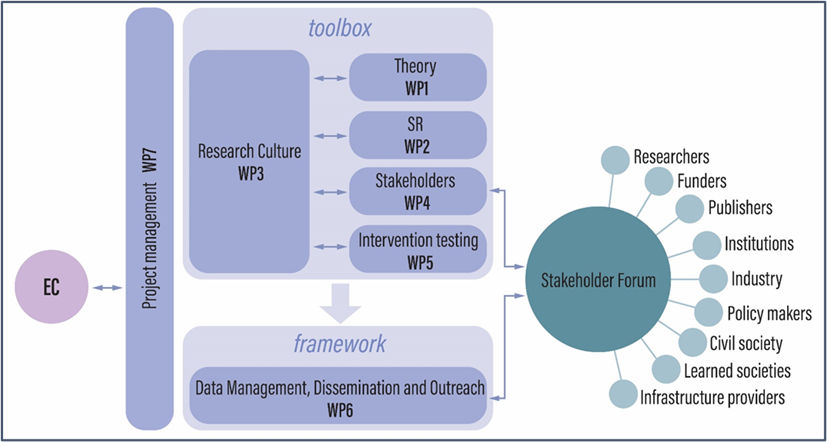
\includegraphics{images/Consortium structure.png}
\caption{Figure 1. Graphical depiction of the iRISE consortium management
structure}
\end{figure}

\hypertarget{project-plan}{%
\subsection{Project Plan}\label{project-plan}}

A well-structured project plan serves as a roadmap to achieve our
objectives and milestones efficiently. This section provides guidance
and descriptions on the iRISE project plan, including work package
descriptions, tasks, milestones and timelines. The \href{https://charitede.sharepoint.com/:b:/r/sites/iRISE/Shared\%20Documents/General/Grant\%20Agreement/GA\%20amendment\%20Sept.\%202023/iRISE_Annex1B_DoA_2023-09-25_v4_clean.pdf?csf=1\&web=1\&e=CGlIBC}{Description of
Action
(DoA)}
and \href{https://charitede.sharepoint.com/:f:/r/sites/iRISE/Shared\%20Documents/General/Grant\%20Agreement/AMD-101094853-4_Nov2023?csf=1\&web=1\&e=cuFpdE}{iRISE Grant
Agreement}
include this information in detail.\\
\textbf{Work Package Descriptions}: Each work package (WP) is a critical
component of the iRISE project. WP descriptions outline the purpose,
scope, and tasks of each AP. Work package leaders and team members
should use these descriptions as a reference for their responsibilities.
Aligning work packages with the overall project objectives is
essential.\\
\textbf{Task Plans}: Tasks are the building blocks of work packages that
describe the individual activities. Individuals are assigned
responsibilities within tasks and clear timelines for each task are set
considering dependencies between tasks and work packages.\\
\textbf{Milestone Definition}: Milestones represent significant project
achievements. They are Specific, Measurable, Achievable, Relevant, and
Time-bound (SMART). Milestones help track progress and ensure alignment
with the project's objectives.\\
\textbf{Budget Plan}: Substantial time and consideration were given to budget
planning for the successful execution of iRISE. The budget plan is
detailed in the Grant Agreement. Eligible expenses and how to monitor
and report on budget use are also detailed in the Grant Agreement and we
encourage consultation with your European Research Office (or
equivalent) to assist with ensuring partners keep within their allocated
budget.\\
\textbf{Risk Management}: It is critical that project risks are identified
and managed, including a description of mitigation plans.\\
\textbf{Change Management}: Over the lifetime of iRISE, things may evolve and
require changes to the project plan. Anticipated changes must be
communicated to the Project Management Office (PMO) as early as possible
and must include details of the requested change with an evaluation of
the impact of changes on project goals and timelines.\\
\textbf{Quality Assurance}: Maintaining the quality of iRISE deliverables is
essential throughout the project's lifecycle. The strategy for quality
control and quality assurance activities is described in further detail
in the Deliverables section of this handbook.\\
\textbf{Collaboration and Communication}: Effective communication and
collaboration are essential for project success. Tools and platforms for
sharing project information and strategies are described in detail in
the Communication and Reporting section of this handbook.

\hypertarget{communication-and-reporting}{%
\section{\texorpdfstring{\textbf{Communication and Reporting}}{Communication and Reporting}}\label{communication-and-reporting}}

\hypertarget{internal-communication}{%
\subsection{Internal communication}\label{internal-communication}}

\hypertarget{emails}{%
\subsubsection{Emails}\label{emails}}

Day-to-day communication will be based on emails. All emails should include ``iRISE'' in the subject header and WP number where appropriate. An overview of available mailing lists and the complete lists can be accessed in the iRISE SharePoint in the \href{https://charitede.sharepoint.com/:w:/r/sites/iRISE/Shared\%20Documents/General/iRISE\%20Mailing\%20List\%20Full.docx?d=w78aadfc66f9b4bdc878dd41138496398\&csf=1\&web=1\&e=xnGHy4}{mailing lists file}. If a person needs to be added/removed from the list (or needs to be added to Microsoft Teams), then each partner should edit the respective list(s) in the mailing lists file.

\hypertarget{meetings}{%
\subsubsection{Meetings}\label{meetings}}

\textbf{WP meetings}: To keep all WP members and project partners up-to-date and coordinate tasks, monthly meetings will be held for each WP. WP leaders will organize and chair the meeting with their WP members. During the first quarter of the project, WP leaders have defined that their monthly meetings will be held according to the information provided in the following table:

\begin{longtable}[]{@{}
  >{\raggedright\arraybackslash}p{(\columnwidth - 2\tabcolsep) * \real{0.2500}}
  >{\raggedright\arraybackslash}p{(\columnwidth - 2\tabcolsep) * \real{0.7500}}@{}}
\toprule()
\begin{minipage}[b]{\linewidth}\raggedright
WP
\end{minipage} & \begin{minipage}[b]{\linewidth}\raggedright
Date/Time (e.g.~First Tuesday of the month 10am CET)
\end{minipage} \\
\midrule()
\endhead
1 & First Friday of month 2:30pm CET (subject to change) \\
2 & Every 14 days (on a Tuesday) 1:00pm CET \\
3 & First Tuesday of a month, 10-11 am CET, intended to be changed to more frequent meetings once the WP starts \\
4 & TBD once WP4 tasks begin \\
5 & Every second Wednesday 10:00-11:00 CET, intended to be changed to monthly meetings after month 6 \\
6 & Scheduled monthly in response to doodle \\
7 & Last Wednesday of the month -- 10:30-11:30 CET \\
SC & Last Wednesday/Thursday of the month every Quarter -- 10:30-12:00 CET \\
\bottomrule()
\end{longtable}

\textbf{SC meetings}: The SC will meet every 3 months (every quarter). SC meetings will be organized and chaired by the PMO. Meetings will be virtual except for those that coincide General Assemblies that will take place in person.\\
In the lead up to each SC meeting, WP leads will be asked to provide a plan for the next 6 months. This plan should include upcoming deliverables, task aims, timeline for each specific step, and areas of priority, integration with other WPs, TIER2 and OSIRIS as well as communication and publication strategy.\\
During less intensive periods or when many partners are absent (e.g., summer), meetings might be held less frequently (e.g., every two months), depending on the project requirements and progress. During busy periods, they may be held more frequently (e.g., every two weeks or upon request).

\hypertarget{microsoft-teams}{%
\subsubsection{Microsoft Teams}\label{microsoft-teams}}

All members should be included in the \href{https://teams.microsoft.com/l/team/19\%3aBeyH-eKopgikP84hU4FuJggrTXugFiipnYUq8krUnAE1\%40thread.tacv2/conversations?groupId=63cd0d10-aa1b-4db9-9bb0-ed23b58ec69b\&tenantId=afe91939-923e-432c-bc66-cbc3ec18d02c}{iRISE Microsoft Teams}, which is hosted by Charité -- Universitätsmedizin Berlin. Individual members are tagged for the WPs in which they are included. The chat function may be used for communication, but important information must be shared via email.

\hypertarget{file-storage}{%
\subsection{File Storage}\label{file-storage}}

The \href{https://charitede.sharepoint.com/sites/iRISE/Shared\%20Documents/Forms/AllItems.aspx}{iRISE SharePoint} that sits behind our Teams page, hosted by Charité -- Universitätsmedizin Berlin, will serve as a platform for storing, sharing and collaborating on documents. All documents must be stored in the corresponding WP section.\\
To ensure version control and facilitate collaborative writing, file links should be used for sharing documents instead of downloaded versions. This will also reduce email traffic. Synchronizing the SharePoint to your computer eases access.

\hypertarget{citation-management}{%
\subsection{Citation Management}\label{citation-management}}

Literature will be shared and managed on an \href{https://www.zotero.org/groups/5148075/irise_library}{iRISE Zotero Library}. Folders can be created for each WP, task or publication as needed. All members have received the following instructions for joining the library:\\
Install Zotero: \url{https://www.zotero.org/download/}\\
Instructions for using group libraries Zotero \textbar{} Groups: \url{https://www.zotero.org/groups/}\\
Install the connector plugin for using Zotero in Microsoft Word and adding references from your browser:\\
\url{https://www.zotero.org/support/word_processor_integration} \url{https://microsoftedge.microsoft.com/addons/detail/nmhdhpibnnopknkmonacoephklnflpho}\strut \\
This allows adding references from your browser to the currently active Zotero library.

\hypertarget{external-communication}{%
\subsection{External communication}\label{external-communication}}

iRISE communications will uphold the values of openness and integrity, and support reproducibility by committing to not sharing unsupported or misleading information. The iRISE \href{https://charitede.sharepoint.com/:w:/r/sites/iRISE/Shared\%20Documents/WP6/iRISE\%20Dissemination\%20Plan_Draft\%201.2.docx?d=w7a63d0ea4a374c1bbe3b7fd98d0c7d2f\&csf=1\&web=1\&e=jY54DT}{Dissemination, Exploitation, and Communication Plan} outlines preliminary strategies for effectively sharing all expected iRISE project outcomes and maximising their impact. All external communication activities (e.g.~events, presentations, and publications) will be collected via the \href{https://charitede.sharepoint.com/:x:/r/sites/iRISE/Shared\%20Documents/WP6/iRISE\%20Dissemination\%20Activity\%20Record.xlsx?d=w47a1cbfaa6c34ab5aee84a6dba643912\&csf=1\&web=1\&e=85BMn0}{Dissemination Activity Record form}, which all members of the Consortium are asked to fill in continuously. All created output will be available under the Creative Commons Attribution 4.0 International (CC BY 4.0) licence.\\
Further detailed information is included in the \href{https://charitede.sharepoint.com/:w:/r/sites/iRISE/Shared\%20Documents/WP6/iRISE\%20Dissemination\%20Plan_Draft\%201.2.docx?d=w7a63d0ea4a374c1bbe3b7fd98d0c7d2f\&csf=1\&web=1\&e=jY54DT}{Dissemination, Exploitation, and Communication Plan}.

\hypertarget{funding-acknowledgement}{%
\subsubsection{Funding Acknowledgement}\label{funding-acknowledgement}}

All iRISE communication materials as well as publications and other outputs must acknowledge EU support by displaying the \href{https://webgate.ec.europa.eu/funding-tenders-opportunities/pages/viewpage.action?pageId=1867972}{European flag (emblem) and funding statement}. Additionally, the following disclaimer must be included:\\
``iRISE receives funding from the European Union's Horizon Europe research and innovation programme under grant agreement No 101094853. Views and opinions expressed are however those of the author(s) only and do not necessarily reflect those of the European Union or the European Research Executive Agency (ERA). Neither the European Union nor the ERA can be held responsible for them. iRISE also receives funding from the Swiss State Secretariat for Education, Research and Innovation (SERI): Direct Funding for Collaborative Projects as part of the transitional measures, and from UK Research and Innovation (UKRI).

\hypertarget{branding}{%
\subsubsection{Branding}\label{branding}}

iRISE will maintain a consistent brand by using our logo, tagline, colour palette and fonts. Details of branding, including colours and fonts, can be found in the \href{https://charitede.sharepoint.com/:w:/r/sites/iRISE/Shared\%20Documents/WP6/iRISE\%20Dissemination\%20Plan_Draft\%201.2.docx?d=w7a63d0ea4a374c1bbe3b7fd98d0c7d2f\&csf=1\&web=1\&e=jY54DT}{Dissemination, Exploitation, and Communication Plan}. The iRISE logo (Figure 2) and its different formats and variants, including logos for each WP can be found in the \href{https://charitede.sharepoint.com/:f:/r/sites/iRISE/Shared\%20Documents/Branding\%20and\%20Website/iRISE\%20Logos/Logos?csf=1\&web=1\&e=mh7pQM}{Logos} Folder. The logo should be included on all presentation and external communication materials.

\begin{figure}
\centering
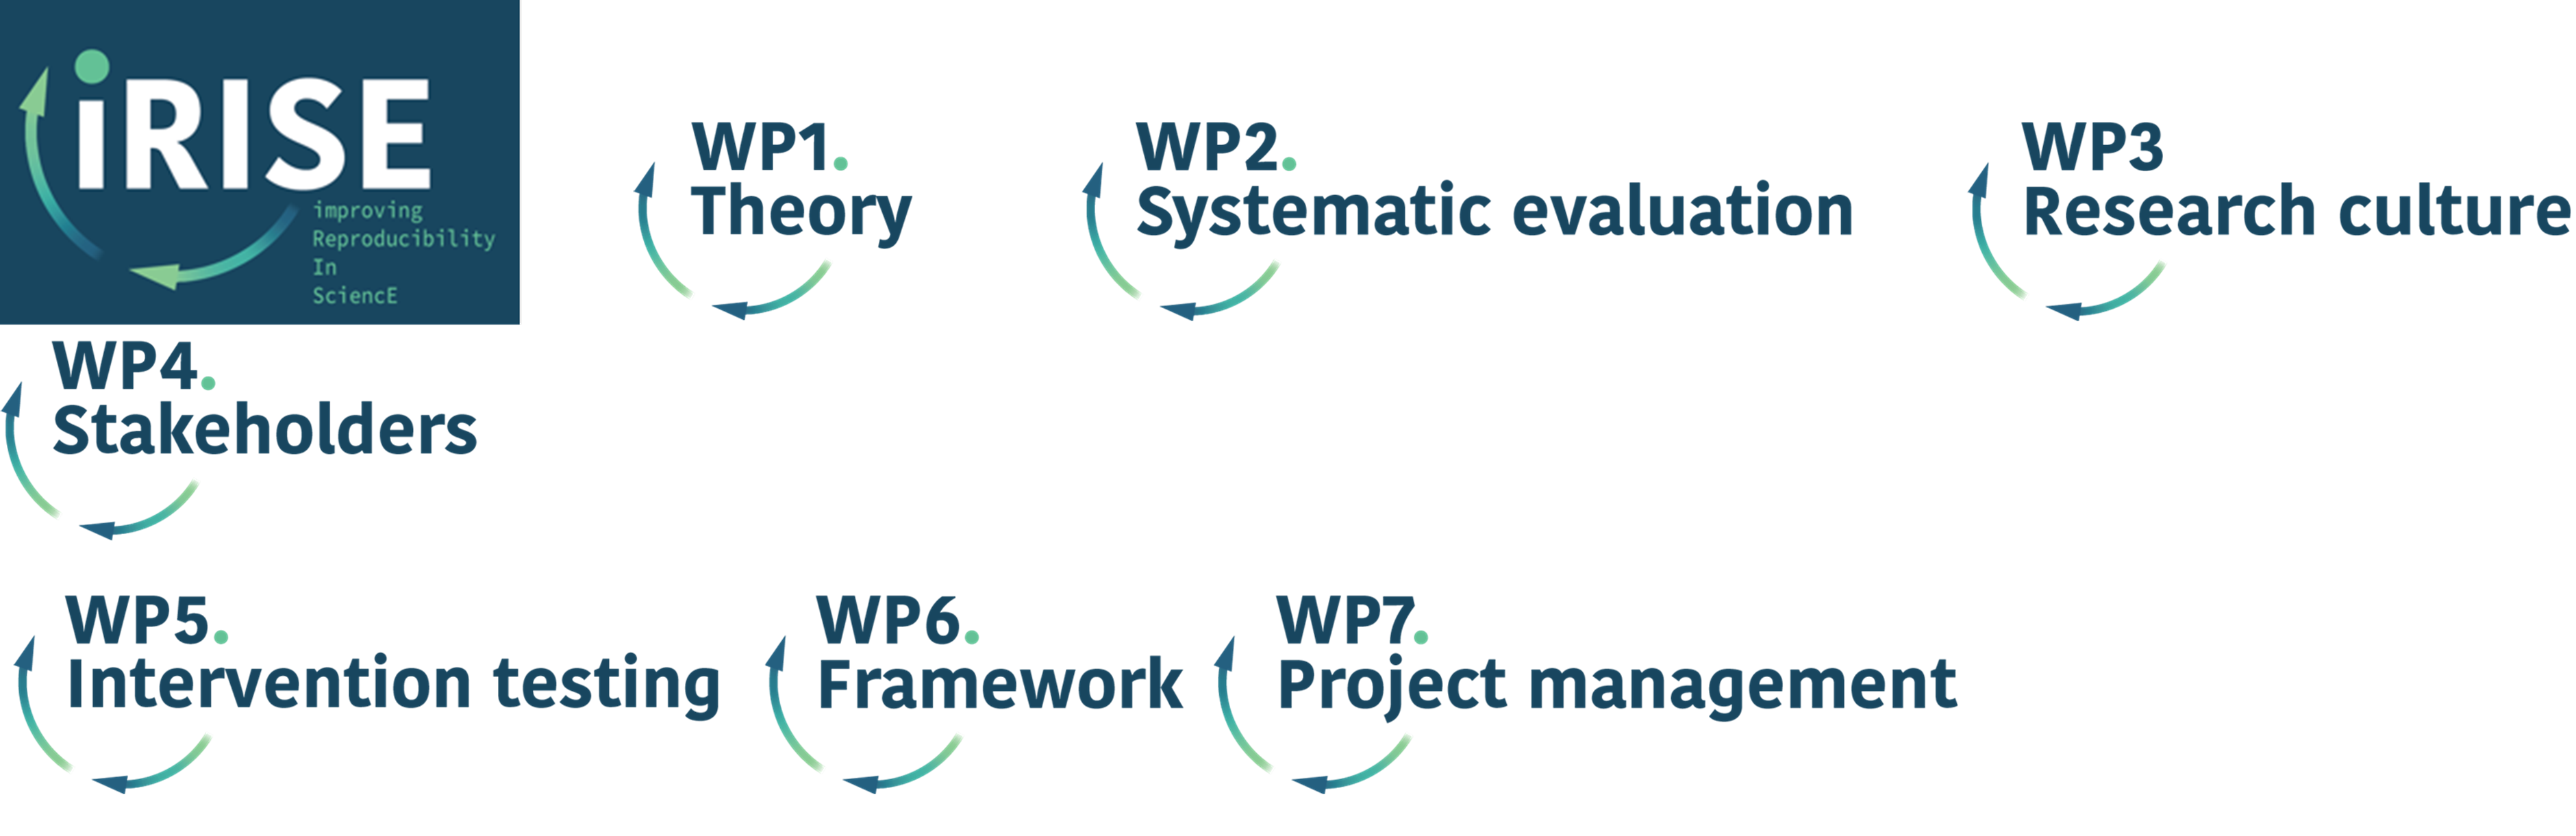
\includegraphics{images/Communication and reporting.png}
\caption{Figure 2: The iRISE logo and individual WP logos}
\end{figure}

\hypertarget{templates-for-deliverables-and-presentations}{%
\subsubsection{Templates for Deliverables and Presentations}\label{templates-for-deliverables-and-presentations}}

All templates are available in the \href{https://charitede.sharepoint.com/:f:/r/sites/iRISE/Shared\%20Documents/General/iRISE\%20Dissemination_Communication_Templates/Templates?csf=1\&web=1\&e=P8QVBa}{General/iRISE Dissemination\_Communication\_Templates} folder.\\
\href{https://charitede.sharepoint.com/:p:/r/sites/iRISE/Shared\%20Documents/General/iRISE\%20Dissemination_Communication_Templates/Templates/PPT\%20Template.pptx?d=w197f096e83fa4576a6f82bdcd51489b2\&csf=1\&web=1\&e=MREwQ4}{PowerPoint} and \href{https://charitede.sharepoint.com/:w:/r/sites/iRISE/Shared\%20Documents/General/iRISE\%20Dissemination_Communication_Templates/Templates/DocTemplate.docx?d=wcb083ece13604791b342b0bb693fe067\&csf=1\&web=1\&e=f61QPR}{Word Doc} templates (including a \href{https://charitede.sharepoint.com/:u:/r/sites/iRISE/Shared\%20Documents/Branding\%20and\%20Website/iRISE.thmx?csf=1\&web=1\&e=fyKrZL}{PowerPoint Theme}) that use the iRISE colour palette, logo and include the required acknowledgment wording are available for presentations and external communication. All presentations in which iRISE results are disseminated must use these branded files (hence, not with, for example, partner institution templates). Other templates may only be used for presentations in which majority of the content is not related to iRISE. Even in these cases, slides with iRISE results must include the logo, and the final slide must acknowledge funding for iRISE as described above. For Deliverables, a \href{https://charitede.sharepoint.com/:w:/r/sites/iRISE/Shared\%20Documents/General/iRISE\%20Dissemination_Communication_Templates/Templates/DeliverableTemplate.docx?d=w4ec2474158ab425f86655df0f923297d\&csf=1\&web=1\&e=drgFm9}{Deliverable Template} is available. Deliverables should not deviate from the structure and style of the template. If any team creates a new item, for example a Poster, and there was no previous template, they will coordinate with WP6 to ensure communication is always conducted respecting the identity of the project.

\hypertarget{website-and-social-media-platforms}{%
\subsubsection{Website and Social Media Platforms}\label{website-and-social-media-platforms}}

The project website is available at \url{https://irise-project.eu/} and presents the project, the team and the SEAB. Additionally, it provides access to all project results and materials.\\
At present, iRISE uses two social media platforms:\\
1. \textbf{X} (formerly Twitter), the handle for the project is \href{https://www.bing.com/ck/a?!\&\&p=aae49b8cd9d6708eJmltdHM9MTY5OTQ4ODAwMCZpZ3VpZD0yZjIzNzQ2Yy1hNzdkLTZiMjEtMDUyYi02NzYzYTYyNTZhYjEmaW5zaWQ9NTE3Nw\&ptn=3\&hsh=3\&fclid=2f23746c-a77d-6b21-052b-6763a6256ab1\&psq=\%40iRISE_EU+twitter\&u=a1aHR0cHM6Ly90d2l0dGVyLmNvbS9pUklTRV9FVQ\&ntb=1}{@iRISE\_EU}\\
2. \textbf{LinkedIn}, which can be found here: \url{https://www.linkedin.com/company/irise-eu/}\\
The social media accounts are managed by WP6. All iRISE consortium members are encouraged to interact with iRISE posts to help boost their reach. Consortium members are also encouraged to create content that can be shared via our social media channels. Please contact Gillian Currie (\href{mailto:gillian.currie@ed.ac.uk}{\nolinkurl{gillian.currie@ed.ac.uk}}) with relevant content.

\hypertarget{internal-reporting-to-project-coordinator}{%
\subsection{Internal Reporting to Project Coordinator}\label{internal-reporting-to-project-coordinator}}

In addition to obligatory reporting to the EC (see \protect\hyperlink{reporting-to-the-european-commission}{Reporting to the European Commission section}), each WP will be asked to provide a work plan every 6 months, and each beneficiary will be asked to provide a financial report every 6 months to the coordinator. All members of the Consortium shall further continuously \href{https://charitede.sharepoint.com/:x:/r/sites/iRISE/Shared\%20Documents/WP6/iRISE\%20Dissemination\%20Activity\%20Record.xlsx?d=w47a1cbfaa6c34ab5aee84a6dba643912\&csf=1\&web=1\&e=9cfBaW}{report any outreach activities at events (conferences, seminars, etc.) as well as publications and datasets related to the project via dedicated reporting forms}, to facilitate periodic reporting about dissemination and communication activities.

\hypertarget{month-wp-plans}{%
\subsubsection{6-Month WP Plans}\label{month-wp-plans}}

All partners will be asked to contribute to WP plans which will be put together at the beginning of each 6-month period, that will be presented at alternating SC meetings. Each WP leader is responsible for collecting contributions from all task leaders and uploading the work plan into the corresponding file on the Teams Environment within 2 weeks after the beginning of each new period (M6, M12, M18, M24, M30). WP leads will be sent a template for completing this information in advance. All WP plans describe the work plan for the following 6-month separately for each task in the WP, including upcoming deliverables, task aims, timeline for each specific step, areas of priority, integration with other WPs as well as communication and publication strategy. The communication strategy describes when and how awareness among the Consortium and external stakeholders will be raised. The publication strategy lists the publications planned for each task, including contributing authors and a preliminary abstract. Reports will further contain a section reporting on achieved results in the previous period, including milestones and deliverables, as well as deviations from the previous plan.

\hypertarget{financial-reporting-every-6-months}{%
\subsubsection{Financial Reporting every 6 Months}\label{financial-reporting-every-6-months}}

Every 6 months, the controlling team at the coordinating institution will further send out an excel-sheet for reporting on financial resources. All partners are asked to report their use of resources in the respective tab of this document.

\hypertarget{data-and-file-management}{%
\section{\texorpdfstring{\textbf{Data and file management}}{Data and file management}}\label{data-and-file-management}}

\hypertarget{file-storage-for-internal-collaboration}{%
\subsection{File Storage for internal collaboration}\label{file-storage-for-internal-collaboration}}

As described above, all documents must be stored and shared in the corresponding WP section of iRISE SharePoint. To ensure version control and facilitate collaborative writing, file links should be used for sharing documents instead of downloaded versions. Synchronizing the SharePoint to your computer eases access.

\hypertarget{data-management-plan}{%
\subsection{Data management plan}\label{data-management-plan}}

The first version of the DMP will be published through DMP online before month 6 {[}link to follow{]}. An internal version of the DMP will be deposited on iRISE Microsoft Teams in the section for WP 6. The DMP is populated with the task-specific information collected in the \href{https://charitede.sharepoint.com/:x:/r/sites/iRISE/_layouts/15/Doc.aspx?action=edit\&sourcedoc=\%7B8fc7f6ef-0e91-450d-b04b-792fd74e205f\%7D\&wdOrigin=TEAMS-WEB.teamsSdk.openFilePreview\&wdExp=TEAMS-CONTROL\&web=1}{DMP table on the iRISE teams}. The plan will be regularly updated. Every six months (starting in September 2024), the core DMP team (Heyard and Currie) will meet with relevant iRISE partners to decide whether updates to the DMP are required. Prior to this meeting, task leads will be sent a survey to collect information on whether the management plan for the data outputs they are responsible for has changed. All task leads must fill in the survey, even if nothing has changed. WP leads are requested to contact the DMP core team via email if major updates to the DMP are required (before the next scheduled meeting).

\hypertarget{minimal-metadata-standards}{%
\subsection{Minimal metadata standards}\label{minimal-metadata-standards}}

All data outputs will be complemented with metadata, as outlined in the DMP. The following elements are required:

\begin{enumerate}
\def\labelenumi{\arabic{enumi}.}
\tightlist
\item
  \textbf{Title}: title describing the data output at hand.\\
\item
  \textbf{Principal Investigator or Creator}: the main person(s) responsible for the intellectual content, with affiliation(s).\\
\item
  \textbf{Contributor(s)}: any other person(s) who contributed to the data output with affiliation(s).\\
\item
  \textbf{Funding}: funding source of the project leading to the data output (iRISE and additional funding sources must be acknowledged here).\\
\item
  \textbf{References and citations}: Citations to relevant work or other objects/material leading to the data output or using the data output. Only cite those articles or material that are important for the data output to be reusable and interpretable. Specifically, if applicable, cite any software or material needed to interact with the data.\\
\item
  \textbf{Summary \textbar{} Description}: A textual description of the aims of data collection and a summary of the data output itself (in the form of a short abstract).\\
\item
  \textbf{Keywords}: List of relevant keywords making the metadata findable.\\
\item
  \textbf{Coverage}: when and where was the data collection - or the project - started and when was it finalized.\\
\item
  \textbf{Date of publication}: Date of data deposition (first -- and new versions)\\
\item
  \textbf{Unit of observation}\\
\item
  \textbf{Population}: information on the population of interest represented or targeted in the data output.\\
\item
  \textbf{Data type and format}: information on the type and format of the data collected.\\
\item
  \textbf{Sampling and weighting}: information on whether any sampling or weighting was used in the data acquisition, and if so, which type or method of sampling and/or weighting was used.\\
\item
  \textbf{Mode of Collection}: information on how the data was collected, on the method used for data collection.\\
\item
  \textbf{DOI}\\
\item
  \textbf{Licenses and restrictions}\\
\item
  \textbf{Ethical considerations}: if ethical approval was needed and acquired, the metadata should link or cite the ethics approval.\\
\item
  \textbf{Description of variables}: if possible, this should be done in a separate code book or data dictionary.
\end{enumerate}

\hypertarget{reporting-to-the-european-commission}{%
\section{\texorpdfstring{\textbf{Reporting to the European Commission}}{Reporting to the European Commission}}\label{reporting-to-the-european-commission}}

Over the course of the project two periodic reports (the latter of which is the final report) must be submitted to the European Commission. They cover the following project periods:

\begin{itemize}
\tightlist
\item
  Period 1: M1-M18 = 1 September 2023 -- 28 February 2025\\
\item
  Period 2: M19-M36 = 1 March 2025 -- 28 August 2026
\end{itemize}

The periodic reports will be submitted by the coordinator within 60 days of the end of each reporting period, which is in M18 and M36 respectively.\\
General reporting principles will be as follows:

\begin{itemize}
\tightlist
\item
  The Project Coordinator will request WP leaders to report on their WP using a generic reporting template provided by the Project Coordinator;\\
\item
  WP leaders will prepare inputs for the periodic report by collecting inputs from their WP task leaders;\\
\item
  The Project Coordinator will combine all this information into a coherent periodic report.\\
\item
  All partners will then review this report.\\
\item
  The Project Coordinator will then revise appropriately and submit to the EC by the required date.\\
\item
  Please note that all partners must keep time records of the hours worked on the action, in accordance with Article 20.1(e) of the Grant Agreement.
\end{itemize}

\hypertarget{periodic-technical-reporting}{%
\subsection{Periodic Technical Reporting}\label{periodic-technical-reporting}}

The periodic technical reports cover the work conducted by the project partners between M1 and M18, and M19 and M36. The periodic reports will follow the official template and will contain the following parts:

\textbf{Part A}: Is created by the participant portal's IT system based on information entered by participants.

\begin{itemize}
\item
  Summary for publication

  \begin{itemize}
  \tightlist
  \item
    Summary of the context and overall objectives of the project\\
  \item
    Work performed from the beginning of the project to the end of the period covered by the report including main results achieved so far\\
  \item
    Progress beyond the state of the art and expected potential impact
  \end{itemize}
\item
  Overview of researchers involved in the project\\
\item
  Deliverables\\
\item
  Milestones\\
\item
  Critical Risks\\
\item
  Project Pathway to Impact\\
\item
  Results Ownership List\\
\item
  Publications\\
\item
  Datasets\\
\item
  Intellectual property rights\\
\item
  Standards\\
\item
  Other results\\
\item
  Dissemination and communication activities\\
\item
  Impact\\
\item
  Research Infrastructure
\end{itemize}

\textbf{Part B}: Part B will be compiled in a Word document within the Teams environment, based on inputs provided by the WP leads and then submitted as one comprehensive report by the coordinator.

\begin{itemize}
\item
  Explanation of the work carried out by the beneficiaries and overview of the progress

  \begin{itemize}
  \tightlist
  \item
    Objectives of the project\\
  \item
    Explanation of the work carried out in each WP\\
  \item
    Impact
  \end{itemize}
\item
  Follow-up of recommendations and comments from previous review(s) (if applicable)\\
\item
  Open Science\\
\item
  Deviations from Description of Action (Annex 1 \& 2) (if applicable)
\end{itemize}

\hypertarget{periodic-financial-reporting}{%
\subsection{Periodic Financial Reporting}\label{periodic-financial-reporting}}

Financial statements cover each partner's cost claim for the previous reporting period. They will be submitted to the European Commission electronically via the participant portal. An individual financial statement (Annex 4 of the \href{https://charitede.sharepoint.com/:f:/r/sites/iRISE/Shared\%20Documents/General/Grant\%20Agreement/AMD-101094853-4_Nov2023?csf=1\&web=1\&e=IRbwUs}{GA}) from each beneficiary will provide an explanation of the use of resources and the information on subcontracting and in-kind contributions provided by third parties from each beneficiary for the reporting period concerned. Before submission, the financial statement must be signed by the financial signatory at each partner institution (FSIGN). The request for interim payment will be also submitted together with the financial statement. If a partner does not submit their financial reporting on time, no interim payment to the respective partner will be made during this period.\\
The individual financial statement must detail the eligible costs (outlined under Article 6 of the \href{https://charitede.sharepoint.com/:f:/r/sites/iRISE/Shared\%20Documents/General/Grant\%20Agreement/AMD-101094853-4_Nov2023?csf=1\&web=1\&e=IRbwUs}{GA}) for each budget category (see Annex 2). Eligible costs include:

\begin{itemize}
\tightlist
\item
  direct personnel costs;\\
\item
  direct costs of subcontracting;\\
\item
  direct costs of providing financial support to third parties;\\
\item
  other direct costs (travel costs, equipment, other goods and services);\\
\item
  indirect costs (flat rate 25\%)
\end{itemize}

All records and supporting documents of costs must be kept as proofs (see article 20 of the \href{https://charitede.sharepoint.com/:f:/r/sites/iRISE/Shared\%20Documents/General/Grant\%20Agreement/AMD-101094853-4_Nov2023?csf=1\&web=1\&e=IRbwUs}{GA}). Further information related to financial management can be found in the EC \href{https://webgate.ec.europa.eu/funding-tenders-opportunities/display/OM/Online+Manual}{Online Manual}.

\textbf{To ensure smooth and accurate financial reporting, iRISE will undertake a ``dry run'' of the financial reporting exercise in Month 6 -- February 2024.}

\hypertarget{continuous-reporting}{%
\subsection{Continuous Reporting}\label{continuous-reporting}}

Continuous Reporting is available from the beginning of the project and can be edited by all beneficiaries in SyGMa (System for Grant Management). A snapshot of the data entered within the tabs for continuous reporting will also be included in the periodic reports when submitted. More information on continuous reporting can be found \href{https://webgate.ec.europa.eu/funding-tenders-opportunities/display/IT/Continuous+Reporting}{here}.

\hypertarget{reporting-on-impact}{%
\subsubsection{Reporting on Impact}\label{reporting-on-impact}}

Different SyGMa tabs (Impact, Impact continuation, Beneficiaries feedback) include questionnaires to monitor and evaluate the Horizon Europe programme performance. There, progress of the impact is recorded.

\begin{itemize}
\tightlist
\item
  Impact questionnaire: collects information about technology readiness, Sustainable Development Goals (SDGs) and citizen engagement
\item
  Impact continuation questionnaire: records information about scientific, societal, environmental and economic impacts of project implementation
\item
  Beneficiaries feedback questionnaire asks about key factors fostering and impeding the impact of the progress of the project
\end{itemize}

\hypertarget{reporting-on-communication-dissemination-and-exploitation}{%
\subsubsection{Reporting on Communication, Dissemination and Exploitation}\label{reporting-on-communication-dissemination-and-exploitation}}

Reporting on communication, dissemination and exploitation follows a qualitative rather than a quantitative approach. Two separate tabs exist in SyGMa on communication and dissemination activities. The main communication and dissemination activities should be added to these tabs, especially when costs were charged to the project. Activities should be described including their purpose, the target audience and their status. It is critical the iRISE consortium members regularly enter details into the \href{https://charitede.sharepoint.com/:x:/r/sites/iRISE/Shared\%20Documents/WP6/iRISE\%20Dissemination\%20Activity\%20Record.xlsx?d=w47a1cbfaa6c34ab5aee84a6dba643912\&csf=1\&web=1\&e=9cfBaW}{Dissemination Activity Record} to facilitate this reporting.\\
Entries can be removed from SyGMa if they have not been included in a periodic report and edited if they have not been included in an intermediate report. The final periodic report must include at least one communication and one dissemination activity with the status ``delivered'' and no activities with the stats ``ongoing'' or ``postponed''.

\hypertarget{reporting-on-project-results}{%
\subsubsection{Reporting on Project Results}\label{reporting-on-project-results}}

Continuous reporting on project results is also required, focusing on content. The according tabs in SyGMa are called ``Results'' and ``Other Results''. Name and type of results is to be recorded, if they are Key Exploitable Results, audience or target groups and steps undertaken towards exploitation and market maturity.

\hypertarget{project-summary}{%
\subsubsection{Project Summary}\label{project-summary}}

The project summary is automatically published in CORDIS with the proposal abstract already filled in. It should be continuously updated when the project produces results. The text should be in a simple language and understandable to externals. Short descriptions intended for wider audience should be included in the ``work performed'' and ``results beyond the state of the art''. Another question is included on the ``policy relevance'' of the project to the policy objectives of the call.

\hypertarget{researchers}{%
\subsubsection{Researchers}\label{researchers}}

The questionnaire on researchers involved in the project can be updated anytime in SyGMa when changes occur within the list of participating researchers. Additions should only be made for researchers as defined in the Frascati Manual and for researchers receiving their salary from other sources who are still contributing to the project's activities. If a researcher does not participate or is removed (especially if their participation was considered very important at the time of the proposal), a justification must be given. Each partner will be responsible for updating the information on the EU's platform as the project progresses, also informing the PMO of such changes. If these modifications also result in a change in Task Leaders, this PM Handbook will also be updated with the latest information, as well as all WP Leads being updated during the SC meetings.

\hypertarget{deliverable-management-and-quality-assurance}{%
\section{\texorpdfstring{\textbf{Deliverable Management and Quality Assurance}}{Deliverable Management and Quality Assurance}}\label{deliverable-management-and-quality-assurance}}

The iRISE SharePoint includes \href{https://charitede.sharepoint.com/:f:/r/sites/iRISE/Shared\%20Documents/General/Deliverables\%20submitted?csf=1\&web=1\&e=i2hJoz}{General/Deliverables Submitted
Folder}.
A subfolder has been created for each deliverable (named
{[}Dx.y\_max3words\_deliverable\_name{]}). All PUBLIC deliverables in iRISE
will automatically be published in CORDIS following submission. This
should be kept in mind when preparing deliverables for submission.

\hypertarget{deliverable-document-structure-and-style}{%
\subsection{Deliverable Document Structure and Style}\label{deliverable-document-structure-and-style}}

Deliverables must use the \href{https://charitede.sharepoint.com/:w:/r/sites/iRISE/Shared\%20Documents/General/iRISE\%20Dissemination_Communication_Templates/Templates/DeliverableTemplate.docx?d=w4ec2474158ab425f86655df0f923297d\&csf=1\&web=1\&e=drgFm9}{Deliverable
Template}.
Its style (including fonts, colours, headers/footers, numbering of
headings) and structure must be maintained. The following general
structure should be followed and is as such provided in the deliverable
template of the project:

\begin{itemize}
\tightlist
\item
  Cover page (project title, title of deliverable, date, lead
  beneficiary, authors, reviewers)\\
\item
  Document Information and Revision History (information table,
  revision history table)\\
\item
  Table of Contents\\
\item
  Executive Summary\\
\item
  List of Abbreviations\\
\item
  Core part\\
\item
  Acknowledgements\\
\item
  References\\
\item
  Annexes (optional)
\end{itemize}

\hypertarget{internal-review-process-and-deadlines-for-deliverables}{%
\subsection{Internal Review Process and Deadlines for Deliverables}\label{internal-review-process-and-deadlines-for-deliverables}}

The lead author (task lead) is responsible for submitting the
deliverable by ensuring the latest version is stored within the
respective folder in Microsoft Teams/SharePoint and informing the
Consortium via email within the deadline (as described below). All
deliverables will be reviewed internally in the Consortium.
Content/research deliverables will be reviewed by two project partners
not or only marginally involved in the creation of the deliverable.
Reviewers must ensure that all content is consistent with the provided
summary, the objectives of the deliverable, are scientifically correct
and of high quality. In addition, the reviewers should also perform
proof-reading and grammar checks. The reviewer must provide comments or
modifications using the track changes features. The assigned reviewers
and deadlines for all deliverables are detailed in Table 2. The \href{https://tasks.office.com/charitede.onmicrosoft.com/en-US/Home/Planner/\#/plantaskboard?groupId=63cd0d10-aa1b-4db9-9bb0-ed23b58ec69b\&planId=P4fliqzuUEeyiZo6z3Z3L5YAAegq}{iRISE
PM
Planner}
also details the deadlines and responsible individuals for each
deliverable and milestone.

The lead author and their partner institution are then responsible for
ensuring that all reviewer comments are addressed in a timely fashion to
ensure submission to the EC by the official delivery date. All
deliverables will be uploaded to the EC Participant Portal by Sarah
McCann. Hence, lead authors should ensure that the final deliverable is
stored within the dedicated Microsoft Teams folder and inform the
coordinating partner \textbf{at least two days} in advance of the
final submission date.

Table 1 presents the timeline for the deliverable review process in
terms of weeks and days before the due date. The due date always
corresponds to the last date of the month number indicated in the
\href{https://charitede.sharepoint.com/:b:/r/sites/iRISE/Shared\%20Documents/General/Grant\%20Agreement/GA\%20amendment\%20Sept.\%202023/iRISE_Annex1B_DoA_2023-09-25_v4_clean.pdf?csf=1\&web=1\&e=CGlIBC}{Description of
Action}.
Meanwhile Table 2 presents the responsible reviewer and partner
institution for each Deliverable. As with the case of a change in
researchers participating in the project, if any of the identified
reviewers ceases to participate in iRISE, the partner institution is
responsible for re-assigning a reviewer within their structure and
propose the change to the project co-coordinators, who will either
approve the change or assign the review to another iRISE member whose
knowledge is adequate for the task at hand.

\emph{\textbf{Table 1}: Timeline for deliverable review process}

\begin{longtable}[]{@{}
  >{\raggedright\arraybackslash}p{(\columnwidth - 2\tabcolsep) * \real{0.3239}}
  >{\raggedright\arraybackslash}p{(\columnwidth - 2\tabcolsep) * \real{0.6761}}@{}}
\toprule()
\endhead
1 calendar month before & Deliverable report is available for review in respective MS Teams folder \\
& WP lead(s) send email to designated reviewers to inform them the doc is ready for review \\
& Corresponding WP mailing list is used to inform all WP members that they are able to review and comment \\
10\textsuperscript{th} of the month & Reviews are available in Teams doc \\
17\textsuperscript{th} of the month & Lead author completes cycle of revisions \\
& Whole consortium is able to comment and give approval \\
2 days before & Final version is available on MS Teams \\
& WP lead(s) do final quality check \\
Due date & Deliverable submitted to the Commission by Sarah \\
\bottomrule()
\end{longtable}

\emph{\textbf{Table 2}: Assigned reviewers and deadlines for deliverables}

\begin{longtable}[]{@{}
  >{\raggedright\arraybackslash}p{(\columnwidth - 14\tabcolsep) * \real{0.1250}}
  >{\raggedright\arraybackslash}p{(\columnwidth - 14\tabcolsep) * \real{0.1250}}
  >{\raggedright\arraybackslash}p{(\columnwidth - 14\tabcolsep) * \real{0.1250}}
  >{\raggedright\arraybackslash}p{(\columnwidth - 14\tabcolsep) * \real{0.1250}}
  >{\raggedright\arraybackslash}p{(\columnwidth - 14\tabcolsep) * \real{0.1250}}
  >{\raggedright\arraybackslash}p{(\columnwidth - 14\tabcolsep) * \real{0.1250}}
  >{\raggedright\arraybackslash}p{(\columnwidth - 14\tabcolsep) * \real{0.1250}}
  >{\raggedright\arraybackslash}p{(\columnwidth - 14\tabcolsep) * \real{0.1250}}@{}}
\toprule()
\endhead
\textbf{ID} & \textbf{Deliverable name} & \textbf{Lead} & \textbf{Type} & \textbf{Due Date} & \textbf{Internal delivery date} & \textbf{R1} & \textbf{R2} \\
D7.1 & Project Website & Mattera (MIK) & DEC & 31/10/2023 & 30/09/2023 & Nilsonne (KI) & - \\
D6.2 & Data Management Plan & Currie (UEDIN) & DMP & 29/02/2024 & 31/01/2024 & Miller (MIK) & McCann (Charité) \\
D6.1 & Dissemination and exploitation Plan & Currie (UEDIN) & R & 29/02/2024 & 31/01/2024 & Zellers (UH) & Sena (UEDIN) \\
D5.1 & Study protocols for interventions registered & Heyard (UZH) & R & 29/02/2024 & 31/01/2024 & Fanelli (HW) & McCann (Charité) \\
D1.1 & Glossary of common terminology resulting from scoping reviews & Würbel (UBERN) & R & 31/05/2024 & 30/04/2024 & Hair (UEDIN) & Sena (UEDIN) \\
D2.1 & Completed iRISE-SOLES of interventions to improve reproducibility & Hair (UEDIN) & DEC & 31/07/2024 & 30/06/2024 & Würbel (UBERN) & Miller (MIK) \\
D2.2 & Registration of protocol for systematic review of interventions that have been tested for effectiveness & McCann (Charité) & R & 31/10/2024 & 30/09/2024 & Gerlach (GoEQIPD) & Heyard (UZH) \\
D3.1 & Interim best practice guidelines for embedding and mainstreaming EDI considerations into tool development and interventions in the reproducibility space & Salholz-Hillel (Charité) & R & 31/01/2025 & 31/12/2024 & Wever (RUMC) & Sena (UEDIN) \\
D1.2 & Interim report with main results from simulation studies, modelling and empirical analyses to diagnose and prevent irreproducibility, and testing of meta-scientific predictions & Fanelli (HW) & R & 31/01/2025 & 31/12/2024 & Wever (RUMC) & McCann (Charité) \\
D6.3 & Dissemination and exploitation including communication activities plan update & Currie (UEDIN) & R & 31/01/2025 & 31/12/2024 & Heyard (UZH) & Sena (UEDIN) \\
D6.4 & Interim policy brief & Currie (UEDIN) & R & 31/01/2025 & 31/12/2024 & Marušić (MFEST) & McCann (Charité) \\
D4.1 & Interim report on facilitators and barriers to implementation of interventions and practices & Marušić (MFEST) & R & 31/01/2025 & 31/12/2024 & Wever (RUMC) & Sena (UEDIN) \\
D4.3 & Final report on facilitators and barriers to implementation of interventions and practices & Marušić (MFEST) & R & 31/01/2026 & 31/12/2025 & Wever (RUMC) & McCann (Charité) \\
D4.2 & Priority list of interventions and practices, integrated in The Embassy of Good Science & Marušić (MFEST) & DEC & 31/01/2026 & 31/12/2025 & Miller (MIK) & Sena (UEDIN) \\
D5.2 & Report on results from automated screening tools intervention & Weissgerber (Charité) & R & 31/01/2026 & 31/12/2025 & Currie (UEDIN) & Sena (UEDIN) \\
D5.3 & Report on results from computational reproducibility review intervention & Nilsonne (KI) & R & 31/01/2026 & 31/12/2025 & Hair (UEDIN) & McCann (Charité) \\
D5.4 & Report on results from EQIPD Quality System intervention & Gerlach (GoEQIPD) & R & 31/01/2026 & 31/12/2025 & Marušić (MFEST) & McCann (Charité) \\
D5.5 & Report on results from statistical interventions analysis & Würbel (UBERN) & R & 31/01/2026 & 31/12/2025 & Fanelli (HW) & Sena (UEDIN) \\
D3.2 & Summary of cross-cutting ``support activities'' throughout the project & Zellers (UH) & R & 30/04/2026 & 30/03/2026 & Nilsonne (KI) & Sena (UEDIN) \\
D6.5 & Online portal of Implementation Guide summaries & Currie (UEDIN) & DEC & 30/04/2026 & 30/03/2026 & Fanelli (HW) & McCann (Charité) \\
D2.3 & Completed systematic reviews of interventions that have been tested for effectiveness & McCann (Charité) & R & 30/04/2026 & 30/03/2026 & Nilsonne (KI) & Miller (MIK) \\
D3.3 & Best practice guidelines for embedding and mainstreaming EDI considerations into tool development and interventions in the reproducibility space & Salholz-Hillel (Charité) & R & 31/05/2026 & 30/04/2026 & Marušić (MFEST) & Sena (UEDIN) \\
D6.8 & Final reflection report of the iRISE experience & Currie (UEDIN) & R & 31/07/2026 & 30/06/2026 & Heyard (UZH) & McCann (Charité) \\
D2.4 & Completed framework to evaluate interventions for reproducibility in the context of systematic reviews & McCann (Charité) & R & 31/07/2026 & 30/06/2026 & Fanelli (HW) & Miller (MIK) \\
D1.3 & Summary report with main results from simulation studies, modelling and empirical analyses to diagnose and prevent irreproducibility, and testing of meta-scientific predictions & Heyard (UZH) & R & 31/07/2026 & 30/06/2026 & Weissgerber (Charité) & Sena (UEDIN) \\
D6.7 & Final policy brief & Currie (UEDIN) & R & 31/07/2026 & 30/06/2026 & Salholz-Hillel (Charité) & McCann (Charité) \\
\bottomrule()
\end{longtable}

\hypertarget{file-naming}{%
\subsection{File Naming}\label{file-naming}}

For the draft phase: Dx.y\_max3words\_deliverable\_name\_DRAFT\_n.0.docx\\
For the review phase: Dx.y\_max3words\_deliverable\_name\_REVIEW\_n.0.docx\\
For the final version, we will use:
iRISE\_Dx.y\_max3words\_deliverable\_name.docx\\
n.0 should start with 1.0 and update in instances where new versions are
saved.\\
Authors and reviewers must be identified in the document revision
history table on the second page of each deliverable.

\hypertarget{overview-of-key-dates}{%
\section{\texorpdfstring{\textbf{Overview of Key Dates}}{Overview of Key Dates}}\label{overview-of-key-dates}}

An overview of key dates for each WP can be found in MS Teams: \href{https://teams.microsoft.com/l/entity/com.microsoft.teamspace.tab.planner/_djb2_msteams_prefix_3069180874?context=\%7B\%22channelId\%22\%3A\%2219\%3ABeyH-eKopgikP84hU4FuJggrTXugFiipnYUq8krUnAE1\%40thread.tacv2\%22\%7D\&groupId=63cd0d10-aa1b-4db9-9bb0-ed23b58ec69b\&tenantId=afe91939-923e-432c-bc66-cbc3ec18d02c}{iRISE Project Management - Deliverables and Milest}.\\
In addition, the \href{https://charitede.sharepoint.com/:w:/r/sites/iRISE/Shared\%20Documents/WP7/Project\%20Management/Coord.\%20documents/iRISE_Gantt_chart.docx?d=we193956c04f94ac7a1c696d1cb8560d1\&csf=1\&web=1\&e=wwhhgQ}{iRISE GANTT Chart} provides an overview of the project's trajectory.

\hypertarget{intellectual-property-and-dissemination}{%
\section{\texorpdfstring{\textbf{Intellectual Property and Dissemination}}{Intellectual Property and Dissemination}}\label{intellectual-property-and-dissemination}}

\hypertarget{intellectual-property}{%
\subsection{Intellectual Property}\label{intellectual-property}}

All information on intellectual property rights and ownership of results are specified in the \href{https://charitede.sharepoint.com/:f:/r/sites/iRISE/Shared\%20Documents/General/Grant\%20Agreement/AMD-101094853-4_Nov2023?csf=1\&web=1\&e=cuFpdE}{iRISE Grant Agreement} under Article 16.

\hypertarget{dissemination-strategies}{%
\subsection{Dissemination Strategies}\label{dissemination-strategies}}

The iRISE \href{https://charitede.sharepoint.com/:w:/r/sites/iRISE/Shared\%20Documents/WP6/iRISE\%20Dissemination\%20Plan_Draft\%201.2.docx?d=w7a63d0ea4a374c1bbe3b7fd98d0c7d2f\&csf=1\&web=1\&e=jY54DT}{Dissemination, Exploitation, and Communication Plan} outlines our preliminary strategies for effectively disseminating all expected iRISE project outcomes and maximising their impact. Additionally, we define our target audiences and how the messages will reach them. We will also describe how we will monitor engagement with iRISE outputs and the effectiveness of our dissemination, exploitation and communication activities.

As part of the strategies for disseminating iRISE project results, publications, and public engagement activities, we have developed guidelines and principles for the publication of research outcomes generated within iRISE. The latest version of our publication policy can be found here: \href{https://charitede.sharepoint.com/:w:/r/sites/iRISE/_layouts/15/Doc.aspx?sourcedoc=\%7BD202FA5E-EDE0-432A-84C6-96659F1B420E\%7D\&file=iRISE_Publication_Policy_2023-09-07_draft_v1.docx\&action=default\&mobileredirect=true}{Publication policy}.

The publication policy aims to ensure transparency, fairness, and proper acknowledgment of contributions while upholding the highest standards of research integrity and publication ethics. In addition, the Dissemination and Commination Plan and DMP will provide further details on the dissemination strategies and detailed activities.

\hypertarget{ethics-and-compliance}{%
\section{\texorpdfstring{\textbf{Ethics and Compliance}}{Ethics and Compliance}}\label{ethics-and-compliance}}

Based on self-assessment (included in \protect\hyperlink{appendix-1-ethical-self-assessment-and-ethical-risks-identification}{Annex 1}) and the initial structure of the Project, four main types of ethical considerations have been identified in iRISE:

\begin{itemize}
\tightlist
\item
  Human\\
\item
  Data Protection
\item
  Scientific Research\\
\item
  Artificial intelligence
\end{itemize}

Our Project involves the participation of researchers, workers, employees, and other stakeholders, including the collection of their personal data. Considering the Project's internal stakeholders, i.e., individuals who are affiliated with any of the project's partners, it is assumed that their participation in all of the projects' activities follows the principles of fair distribution of benefits and burdens, the respect for people and human dignity, their rights and personal interests, as well as their free, informed consent to partake in the Project.

Moreover, iRISE involves individuals who are not part of the participants' staff (beneficiaries, affiliated entities, associated partners, subcontractors, etc.). Participation in this Project will be entirely voluntary. External participants' informed consent will be obtained, and advised on how any data they provide will be treated. The treatment of the latter is dealt with in detail in the Data Management Plan (DMP). The EU Ethics and data protection decision tree were implemented to identify ethics issues, together with the Horizon Europe Programme Guide V.3.0\footnote{For further details see the EU Programme Guide V.3.0: \url{https://ec.europa.eu/info/funding-tenders/opportunities/docs/2021-2027/horizon/guidance/programme-guide_horizon_en.pdf}}, specifically the Ethics and Integrity section.

The primary sources of EU and international law are directly linked to the Charter of Fundamental Rights of the European Union, the European Convention on Human Rights (ECHR), and the UN Convention on the Rights of Persons with Disabilities (UNCRPD). This also includes its protocols and other texts, which are included in the reference section and directly relate to:

\begin{enumerate}
\def\labelenumi{\arabic{enumi}.}
\tightlist
\item
  EU Charter of Fundamental Rights\\
\item
  European Convention for the Protection of Human Rights and Fundamental Freedoms and its Supplementary Protocols.\\
\item
  European Code of Conduct for Research Integrity of ALLEA (All European Academies)\\
\item
  EU Regulation 2016/679 Protection of natural persons concerning the processing of personal data and the free movement of such data - General Data Protection Regulation (GDPR)\\
\item
  Swiss New Federal Act on Data Protection, in alignment with the EU's GDPR\\
\item
  UK Equality Act\\
\item
  UK Human Rights Act\\
\item
  UK Consumer Rights legislation\\
\item
  UK data protection laws
\end{enumerate}

The EU rules for data protection and safeguarding ethical principles have been consulted and respected, including fundamental ethical principles. Article 8 of the EU Charter of Fundamental Rights\footnote{For further reference see the definitions within Article 8 of the EU Charter of Fundamental Rights: \url{http://fra.europa.eu/en/eu-charter/article/8-protection-personal-data}} stipulates that everyone in the EU has the right to the protection of personal data concerning themselves, access to data which has been collected concerning them, and the right to rectify it. The EU General Data Protection Regulation (GDPR) expands this, stipulating the right to erasure. All relevant national, EU and international legislation was consulted during the elaboration of the DMP as well as this document.

No research in this Project will involve Human Embryonic Stem Cells, Human embryos or human foetal tissues/cells, animals, plants, or other biological entities tampering with or modifying the environment. Furthermore, at the release of this ethics requirements document, no Artificial Intelligence usage was identified neither as a core part of the development of any task within the Project nor as a tool implemented within any of the partner institution's SOPs. Therefore, it was not considered as an ethical issue.

Lastly, scientific research was the third type of potential risk linked to ethical issues. In this context, adequately gathering data, implementing the most suitable methodological approach, providing detailed and trustworthy results, as well as not incurring any plagiarism, subcontracting, or non-ethical approaches are at the core of iRISE's commitment to upholding high ethical research standards by adhering to the European Code of Conduct for Research Integrity (ECCRI).

\hypertarget{responsible-research-practice}{%
\subsection{Responsible research practice}\label{responsible-research-practice}}

iRISE commits to the highest ethical standards and to follow the \href{https://allea.org/wp-content/uploads/2023/06/European-Code-of-Conduct-Revised-Edition-2023.pdf}{ALLEA European Code of Conduct for research integrity}. Responsibility for adhering to these principles lies primarily with the WP leads. In addition, the Project Coordinator and Project Manager will monitor adherence based on the reporting provided during SC meetings.

\hypertarget{compliance-with-horizon-europe-ethical-standards}{%
\subsection{Compliance with Horizon Europe ethical standards}\label{compliance-with-horizon-europe-ethical-standards}}

iRISE is carried out in line with the highest ethical standards and the applicable EU, international and national law on ethical principles. Consortium members commit to and ensure the respect of basic EU values (such as respect for human dignity, freedom, democracy, equality, the rule of law and human rights, including the rights of minorities). The Consortium and the project coordinator have long-standing experience in managing and working in the context of the EU Research and Innovation Framework Programs and other EU projects engaging different stakeholders and communities.

All beneficiaries of iRISE have been made aware of the ethical principles adopted during the project activities, have participated in the compilation and drafting of this document, and commit to following policies and procedures, as well as complying with the obligations herein disclosed. The Consortium ensures compliance with applicable international, EU and national laws of the iRISE involved partners. It includes the ethical regulations that the EU applies to funded projects, the general ethical recommendations in force in EU countries and the laws applied to sectors that have implicit ethical problems.

The beneficiaries must act in compliance with ethical principles (including the highest standards of research integrity) and - applicable EU, international and national law as stated in the above sections of this document. No funding can be granted for prohibited activities in all Member States within or outside the EU. No funding can be granted in a Member State for an activity forbidden in that Member State. The beneficiaries must pay particular attention to the principle of proportionality, the right to privacy, the right to the protection of personal data, the right to the physical and mental integrity of persons, the right to non-discrimination, the need to ensure the protection of the environment and high levels of human health protection\footnote{For further details see the EU definition on Data Protection, Necessity and Proportionality: \url{https://edps.europa.eu/data-protection/our-work/subjects/necessity-proportionality_en}}. The beneficiaries must ensure that the activities under the action focus exclusively on civil applications.

Additionally, the Project will be carried out with minimal environmental impact, in alignment with the EU's objectives for 2050, including but not limited to the EU Green Deal and the EU Taxonomy\footnote{For further details see the EU definition of objectives towards achieving the EU Green Deal: \href{https://commission.europa.eu/strategy-and-policy/priorities-2019-2024/european-green-deal_en\#:~:text=The\%20European\%20Green\%20Deal\%20will\%20improve\%20the\%20well\%2Dbeing\%20and,healthy\%20and\%20affordable\%20food}{https://commission.europa.eu/strategy-and-policy/priorities-2019-2024/european-green-deal\_en\#:\textasciitilde:text=The\%20European\%20Green\%20Deal\%20will\%20improve\%20the\%20well\%2Dbeing\%20and,healthy\%20and\%20affordable\%20foo}}. In this context, printing will be limited to the essential elements, always using certified paper (i.e., Forest Stewarship Council). Employees working on iRISE-related tasks or WPs will be able to carry out their tasks, wherever possible and in accordance with the partner institutions' internal Human Resources policies in a flexible work-from-home schedule, thus reducing CO2 emissions and limiting negative environmental impact. Following the Furthermore, travelling will be limited to the agreements established within the Grant Agreement (\href{https://charitede.sharepoint.com/:f:/r/sites/iRISE/Shared\%20Documents/General/Grant\%20Agreement/AMD-101094853-4_Nov2023?csf=1\&web=1\&e=IRbwUs}{GA}) to ensure proper deployment of the Project's activities while limiting the negative environmental impact of these actions.

\hypertarget{artificial-intelligence}{%
\subsection{Artificial Intelligence}\label{artificial-intelligence}}

The iRISE consortium will be using artificial intelligence as one of the tools that will support the various tasks, activities and WP milestones and deliverables. To ensure adequate compliance and limiting any potential ethical risks, the AI specific Ethics and Compliance, as well as Data Management Policy using this tool will be detailed in the iRISE Data Management Plan. In this document, details of the scope and usage of AI will be determined, related risks will be identified, and a detailed guide on risk management and ethical risk mitigation will be provided.
Any issues addressing ethical concerns and AI were identified in the self-assessment included in Annex 1 of this document.

\hypertarget{conflict-resolution-policy}{%
\subsection{Conflict resolution policy}\label{conflict-resolution-policy}}

The iRISE consortium agrees on a fair and transparent framework for addressing conflicts that may arise within the project. The conflict resolution policy aims to ensure effective and respectful resolution processes, promoting a harmonious and collaborative environment among consortium members.\\
The current version can be found here: \href{https://charitede.sharepoint.com/:w:/r/sites/iRISE/Shared\%20Documents/WP7/Project\%20Management/iRISE_Conflict_Resolution_Policy_2023-09-07_draft_v1.docx?d=w8c6c4a152a9046dab8a06017a0b97944\&csf=1\&web=1\&e=Nhj4lf}{iRISE\_Conflict\_Resolution\_Policy\_2023-09-07\_draft\_v1.docx}

\hypertarget{risk-management}{%
\subsection{Risk Management}\label{risk-management}}

The consortium members have pre-identified risks and developed preliminary mitigation strategies for each WP, which can be found in the \href{https://charitede.sharepoint.com/:f:/r/sites/iRISE/Shared\%20Documents/WP7/Project\%20Management/Risk\%20Assessments?csf=1\&web=1\&e=v2Nm3v}{Risk Assessment folder}.

WP leads, in collaboration with task leads, will be required to undertake a formal risk assessment every six months that is presented at alternating SC meeting. Potential issues, contingencies and mitigation strategies must be assessed and described for each task. The potential source of the risk should also be considered (i.e technical, financial, operational, and external factors).

Risk assessments should be presented in a Risk Matrix, that includes description of the potential impact of identified risks on project objectives and the probability of each risk occurring.

It is important that insights from risk management are used to improve future activities and execution, and there is ongoing learning from risk events.

Further information on risk management strategies can also be found in the Data Management Plan.

\hypertarget{key-performance-indicators-for-impact}{%
\section{\texorpdfstring{\textbf{Key Performance Indicators for Impact}}{Key Performance Indicators for Impact}}\label{key-performance-indicators-for-impact}}

The major key performance indicators for impact for iRISE are listed in Table 4. The pilot activities will be revised in accordance with the evolving co-creation strategy. Corresponding performance indicators might therefore be subject to change and in some instances, they are being defined during M1-5 of the project, hence at the time of the initial publication of this PM Handbook they are not complete. The project coordinator will monitor reasonable progress towards the key performance indicators throughout the project.\\

A detailed description of iRISE's pathway to impact can be found in the \href{https://charitede.sharepoint.com/:b:/r/sites/iRISE/Shared\%20Documents/General/Grant\%20Agreement/Amendment\%20-\%20AMD-101094853-4_Grant\%20Agreement\%20iRISE.pdf?csf=1\&web=1\&e=SqVvdc}{iRISE Grant Agreement}.

\emph{\textbf{Table 4}: Key Performance Indicators for Impact}

\begin{longtable}[]{@{}
  >{\raggedright\arraybackslash}p{(\columnwidth - 4\tabcolsep) * \real{0.5205}}
  >{\raggedright\arraybackslash}p{(\columnwidth - 4\tabcolsep) * \real{0.3767}}
  >{\raggedright\arraybackslash}p{(\columnwidth - 4\tabcolsep) * \real{0.0959}}@{}}
\toprule()
\endhead
& \textbf{Success measure} & \textbf{KPI} \\
\textbf{Pilot activities} & & \\
Structured understanding of reproducibility & Glossary & \\
& Theory Output & \\
Catalogue interventions to improve reproducibility across all disciplines & & \\
Evidence-based guidelines of best practice & No.~of final guidelines published & \\
Assessment and summary of interventions' effectiveness & Systematic reviews & \\
& No.~of interventions tested, integrating an EDI lens & 4 \\
\textbf{Dissemination} & & \\
Protocols and study results & No.~of Review Protocols registered & \\
& No.~Study Protocols registered & \\
Open knowledge base & & \\
iRISE-SOLES & & \\
iRISE Framework & & \\
Training materials & & \\
Social media & No.~of Press Releases & \\
& No.~of X posts & \\
Website & No.~of Visits & \\
\bottomrule()
\end{longtable}

\hypertarget{references-and-further-reading}{%
\section{\texorpdfstring{\textbf{References and Further Reading}}{References and Further Reading}}\label{references-and-further-reading}}

ALLEA (2023) The European Code of Conduct for Research Integrity -- Revised Edition 2023. Berlin. DOI 10.26356/ECOC\\
European Commision (2023) EU Grants: HE Programme Guide -- Version 4.0. \url{https://ec.europa.eu/info/funding-tenders/opportunities/docs/2021-2027/horizon/guidance/programme-guide_horizon_en.pdf}\\
European Commission. The European Green Deal. \url{https://commission.europa.eu/strategy-and-policy/priorities-2019-2024/european-green-deal_en\#:~:text=The\%20European\%20Green\%20Deal\%20will\%20improve\%20the\%20well-being\%20and,healthy\%20and\%20affordable\%20food}\\
European Data Protection Supervisor -- Necessity \& Proportionality. \url{https://edps.europa.eu/data-protection/our-work/subjects/necessity-proportionality_en}\\
European Union Agency for Fundamental Rights. Article 8 -- Protection of personal data. \emph{EU Charta of Fundamental Rights}. \url{http://fra.europa.eu/en/eu-charter/article/8-protection-personal-data}.

\hypertarget{appendix-1-ethical-self-assessment-and-ethical-risks-identification}{%
\section{\texorpdfstring{\textbf{Appendix 1: Ethical Self-Assessment and Ethical Risks Identification}}{Appendix 1: Ethical Self-Assessment and Ethical Risks Identification}}\label{appendix-1-ethical-self-assessment-and-ethical-risks-identification}}

\hypertarget{ethics-self-assessment}{%
\subsection{Ethics self-assessment}\label{ethics-self-assessment}}

\begin{longtable}[]{@{}
  >{\raggedright\arraybackslash}p{(\columnwidth - 10\tabcolsep) * \real{0.2523}}
  >{\raggedright\arraybackslash}p{(\columnwidth - 10\tabcolsep) * \real{0.1833}}
  >{\raggedright\arraybackslash}p{(\columnwidth - 10\tabcolsep) * \real{0.0093}}
  >{\raggedright\arraybackslash}p{(\columnwidth - 10\tabcolsep) * \real{0.0093}}
  >{\raggedright\arraybackslash}p{(\columnwidth - 10\tabcolsep) * \real{0.3095}}
  >{\raggedright\arraybackslash}p{(\columnwidth - 10\tabcolsep) * \real{0.2330}}@{}}
\toprule()
\endhead
\textbf{Ethical Areas inherent to the Project} & & \textbf{Yes} & \textbf{No} & \textbf{Information to be provided in the proposal} & \textbf{Documents to be kept on file and provided upon request} \\
HUMANS & & & & & \\
Does your activity involve human participants? & & X & & & \\
If yes & Are they volunteers? & X & & Participation from members of partner institutions is managed by each partner following ethical guidelines and voluntary adhesion to iRISE while external stakeholders will voluntarily sign an informed explicit consent to partake in iRISE. & Signed consent for external participants. \\
& Are they healthy volunteers for medical studies? & & X & & \\
& Are they patients for medical studies? & & X & & \\
& Are they potentially vulnerable individuals or groups? & & X & & \\
& Are they children/minors? & & X & If this were to change throughout the Project, it is necessary to require explicit consent from parents following the same procedure as for individual adult's consent. & \\
& Are there other persons unable to give informed consent? & & X & & \\
Does your activity involve interventions (physical also including imagining technology, behavioural treatments, tracking and tracing, etc.) on the study of participants? & & & X & & \\
If yes & Does it involve invasive techniques (e.g., collection of human cells or tissues, surgical or medical interventions, invasive studies on the brain, TMS, etc.)? & N/A & & & \\
& Does it involve collection of biological samples? & N/A & & & \\
Does your activity involve conducting a clinical study as defined by the Clinical Trial - Regulation 536/2014 (using pharmaceuticals, biologicals, radiopharmaceuticals, or advanced therapy medicinal products)? & & N/A & & & \\
PROTECTION OF PERSONAL DATA & & & & & \\
Does your activity involve processing of personal data? & & X & & Detailed information regarding iRISE's specific data management included in the Data Management Plan & DMP (including Data Protection Impact Assessment)

Informed consent forms and information sheets \\
If yes & Does it involve the processing of special categories of personal data (e.g., sexual lifestyle, ethnicity, genetic, biometric and health data, political opinion, religious or philosophical beliefs)? & X & & WP3 is interested in equity, diversity and inclusion, and research culture and the impact of these domains on reproducibility. These exercises will therefore include collection and assessment of the impact of gender and potentially ethnicity in the reproducibility domain. & \\
& Does it involve processing of genetic, biometric or health data? & & X & & Declaration of confirming compliance with the laws of the country where the data will be collected. \\
& Does it involve profiling, systematic monitoring of individuals, or processing of large-scale of special categories of data or intrusive methods of data processing (such as surveillance, geolocation tracking, etc.)? & & X & Details of the methods used for tracking/profiling, assessment of the ethics risks related to those data processing operations, explanation as to how the rights/freedoms of the participants/subjects will be safeguarded and how they will be informed. & Opinion of the data controller for conducting DPIA - DMP \\
Does your activity involve further processing of previously collected personal data (including use of pre-existing data sets or sources, merging existing data sets)? & & & X & Details of the original data set, including how rights will be safeguarded, how processed data is limited to the purposes of the Project and relevant to its objectives, and/or justification why data will not be anonymised or pseudonymised (if relevant) & Confirmation that the data controller has a lawful basis for the data processing and adequate technical/organisational measures are in place to safeguard the rights of the data subjects including permission by the owner/manager of the data sets (e.g.~social media databases)

Informed consent/information sheets and other applicable documents \\
Is it planned to import personal data (data transfer) from non-EU countries into the EU or from a non-EU country to another non-EU country? & & & X & Details of the types of personal data and countries involved & Confirmation of compliance with the laws of the country in which the data was collected \\
Is it planned to export personal data (data transfer) from non-EU countries into the EU or from a non-EU country to another non-EU country? & & & X & Details of the types of personal data and countries involved & Confirmation of compliance with the laws of the country in which the data was collected \\
Does your activity involve the processing of personal data related to criminal convictions or offenses? & & & X & & \\
6 THIRD COUNTRIES & & & & & \\
Will some of the activities be carried out in non-EU countries? & & X & & The consortium includes members located in Switzerland and in the UK, who follow the same legal frameworks and protection of data and ethical values as EU nations, therefore it is not deemed as a risk to have these organizations involved in some of the projects' tasks. & \\
Do the activities undertaken in these countries raise potential ethics issues? & & & X & Countries/materials involved & Copies of ethics approvals and other authorisations or notifications (if required) and confirmation that the activity could have been legally carried out in an EU country \\
Is it planned to use local resources? (e.g., animal/human tissue samples, genetic material, live animals, human remains, materials of historical value, endangered fauna/flora samples, etc.) & & & X & Details on the type of local resources to be used and modalities & \\
Is it planned to import any material other than data from non-EU countries into the EU or from a non-EU country to another EU country? & & & X & Countries/materials involved & Export licenses/Material Transfer Agreement (MTA) \\
Is it planned to export any material other than data from non-EU countries into the EU or from a non-EU country to another EU country? & & & X & Countries/materials involved & Export licenses/Material Transfer Agreement (MTA) \\
Does your activity involve low and/or lower-middle income countries? & & & X & & \\
ARTIFICIAL INTELLIGENCE AND OTHER ETHICAL ISSUES & & & & & \\
Does this activity involve the development, deployment and/or use of Artificial Intelligence-based systems? & & ~X & & Machine learning classifiers will be used in WP2 to classify research articles, describing whether they are primary research and details of the experimental design and context. The classier will trained using human decisions by members of the consortium. We will describe how machine learning has been used to classify studies, including details of its performance. & \\
Could the AI based system/technique potentially stigmatise or discriminate against people (e.g.~based on sex, race, ethnic or social origin, age, genetic features, disability, sexual orientation, language, religion or belief, membership to a political group, or membership to a national minority)? & & X & & & \\
Does the AI system/technique interact, replace or influence human decision-making processes (e.g.~issues affecting human life, health, well-being or human rights, or economic, social or political decisions)? & & X & & & \\
Does the AI system/technique have the potential to lead to negative social (e.g.~on democracy, media, labour market, freedoms, educational choices, mass surveillance) and/or environmental impacts either through intended applications or plausible alternative uses? & & X & ~X & & \\
Does this activity involve the use of AI in a weapon system? & & ~X & & & \\
Does the AI to be developed/used in the Project raise any other ethical issues not covered by the questions above (e.g., subliminal, covert or deceptive AI, AI that is used to stimulate addictive behaviors, lifelike humanoid robots, etc.)? & & X & & & \\
Are there any other ethics issues that should be taken into consideration? Please specify & & ~X & & & \\
\bottomrule()
\end{longtable}

\end{document}
